\documentclass[12pt]{article}

% 
%\usepackage{showkeys}
%\usepackage{drftcite}
\usepackage{exscale,relsize}
\usepackage{amsmath}
\usepackage{amsfonts}
\usepackage[hidelinks]{hyperref}
\usepackage{amssymb}
\usepackage{calc}
\usepackage{theorem}
\usepackage{pifont}      % needed by dingautolist
\usepackage{array}
\usepackage{color}
\usepackage{enumerate}
\usepackage{bbm}
\usepackage{graphicx}
\usepackage{float}
\usepackage{subfigure}




% FORMATTING ===================================================================
\oddsidemargin -0.1cm
\textwidth  16.5cm
\topmargin  0.0cm
\headheight 0.0cm
\textheight 21.0cm
\parindent  4mm
\parskip    10pt
%\parskip    8pt
\tolerance  3000

% MATH SYMBOLS =================================================================


% These are Heniz's notations. 
\newcommand{\To}{\ensuremath{\rightrightarrows}}
\newcommand{\GX}{\ensuremath{\Gamma}}
\newcommand{\mal}{\ensuremath{\mathfrak{m}}}
\newcommand{\mumu}{\ensuremath{{\mu\mu}}}
\newcommand{\paver}{\ensuremath{\mathcal{P}}}
\newcommand{\ZZZ}{\ensuremath{{X \times X^*}}}
\newcommand{\RRR}{\ensuremath{{\RR \times \RR}}}
\newcommand{\todo}{\hookrightarrow\textsf{TO DO:}}

\newcommand{\emp}{\ensuremath{\varnothing}}
%\newcommand{\la}{\ensuremath{\langle}}
%\newcommand{\ra}{\ensuremath{\rangle}}
\newcommand{\infconv}{\ensuremath{\mbox{\small$\,\square\,$}}}
\newcommand{\pscal}{\ensuremath{\scal{\cdot}{\cdot}}}
\newcommand{\Tt}{\ensuremath{\mathfrak{T}}}
\newcommand{\YY}{\ensuremath{\mathcal Y}}
\newcommand{\XX}{\ensuremath{\mathcal X}}
\newcommand{\HH}{\ensuremath{\mathcal H}}
\newcommand{\XP}{\ensuremath{\mathcal X}^*}
\newcommand{\st}{\ensuremath{\;|\;}}
\newcommand{\zeroun}{\ensuremath{\left]0,1\right[}}

\newcommand{\lev}[1]{\ensuremath{\mathrm{lev}_{\leq #1}\:}}
\newcommand{\moyo}[2]{\ensuremath{\sideset{_{#2}}{}{\operatorname{}}\!#1}}
\newcommand{\pair}[2]{\left\langle{{#1},{#2}}\right\rangle}
%\newcommand{\scal}[2]{\left.\left\langle{#1}\:\right| {#2}  \right\rangle}
\newcommand{\scal}[2]{\langle{{#1},{#2}}\rangle}
\newcommand{\Scal}[2]{\left\langle{{#1},{#2}}\right\rangle}
%\newcommand{\scal}[2]{\braket{ {#1},{#2}}}

\newcommand{\yosida}{\ensuremath{ \; {}^}}
\newcommand{\exi}{\ensuremath{\exists\,}}
\newcommand{\GG}{\ensuremath{\mathcal G}}
\newcommand{\RR}{\ensuremath{\mathbb R}}
\newcommand{\SSS}{\ensuremath{\mathbb S}}
\newcommand{\CC}{\ensuremath{\mathbb C}}
\newcommand{\Real}{\ensuremath{\mathrm{Re}\,}}
\newcommand{\ii}{\ensuremath{\mathrm i}}
\newcommand{\RP}{\ensuremath{\left[0,+\infty\right[}}
\newcommand{\RPX}{\ensuremath{\left[0,+\infty\right]}}
\newcommand{\RPP}{\ensuremath{\,\left]0,+\infty\right[}}
\newcommand{\RX}{\ensuremath{\,\left]-\infty,+\infty\right]}}
\newcommand{\RXX}{\ensuremath{\,\left[-\infty,+\infty\right]}}
\newcommand{\KK}{\ensuremath{\mathbb K}}
\newcommand{\NN}{\ensuremath{\mathbb N}}
\newcommand{\nnn}{\ensuremath{{n \in \NN}}}
\newcommand{\thalb}{\ensuremath{\tfrac{1}{2}}}
\newcommand{\pfrac}[2]{\ensuremath{\mathlarger{\tfrac{#1}{#2}}}}
\newcommand{\zo}{\ensuremath{{\left]0,1\right]}}}
\newcommand{\lzo}{\ensuremath{{\lambda \in \left]0,1\right]}}}
%\newcommand{\toppsepp}{\setlength{\partopsep}{-5pt}}
\newcommand{\menge}[2]{\big\{{#1} \mid {#2}\big\}}


% MATH OPERATORS ===============================================================
% \newcommand{\monos}{\ensuremath{\mathcal M}}
\newcommand{\DD}{\operatorname{dom}f}
\newcommand{\IDD}{\ensuremath{\operatorname{int}\operatorname{dom}f}}
\newcommand{\CDD}{\ensuremath{\overline{\operatorname{dom}}\,f}}
\newcommand{\clspan}{\ensuremath{\overline{\operatorname{span}}}}
\newcommand{\cone}{\ensuremath{\operatorname{cone}}}
\newcommand{\dom}{\ensuremath{\operatorname{dom}}}
\newcommand{\closu}{\ensuremath{\operatorname{cl}}}
\newcommand{\cont}{\ensuremath{\operatorname{cont}}}
\newcommand{\mons}{\ensuremath{\mathcal{A}}}
\newcommand{\gra}{\ensuremath{\operatorname{gra}}}
\newcommand{\epi}{\ensuremath{\operatorname{epi}}}
\newcommand{\prox}{\ensuremath{\operatorname{Prox}_{\mu}}}
\newcommand{\hprox}{\ensuremath{\operatorname{prox}}}
\newcommand{\intdom}{\ensuremath{\operatorname{int}\operatorname{dom}}\,}
\newcommand{\inte}{\ensuremath{\operatorname{int}}}
\newcommand{\sri}{\ensuremath{\operatorname{sri}}}
\newcommand{\reli}{\ensuremath{\operatorname{ri}}}
\newcommand{\cart}{\ensuremath{\mbox{\LARGE{$\times$}}}}


\newcommand{\average}{\ensuremath{\mathcal{R}_{\mu}({\bf A},{\boldsymbol \lambda})}}
\newcommand{\averagebar}{\ensuremath{\mathcal{R}_{1}({\bf A},\bar{\lambda})}}
\newcommand{\averageonelambda}{\ensuremath{\mathcal{R}({\bf A},{\boldsymbol \lambda})}}
\newcommand{\averageonehalf}{\ensuremath{\mathcal{R}_{1}(A,1/2)}}
\newcommand{\averageinverse}{\ensuremath{\mathcal{R}_{\mu^{-1}}({\bf A}^{-1},{\boldsymbol \lambda})}}
\newcommand{\averageoneinverse}{\ensuremath{\mathcal{R}({\bf A}^{-1},{\boldsymbol \lambda})}}
\newcommand{\averagef}{\ensuremath{\mathcal{P}_{\mu}(f,\lambda)}}
\newcommand{\averagefone}{\ensuremath{\mathcal{P}_{1}(f,\lambda)}}
\newcommand{\averagefd}{\ensuremath{\mathcal{P}_{\mu}((f_{1},\ldots, f_{n}),(\lambda_{1},\ldots, \lambda_{n}))}}
\newcommand{\averagefik}{\ensuremath{\mathcal{P}_{\mu_{k}}((f_{1,k},\ldots,f_{n,k}),
(\lambda_{1,k},\ldots,\lambda_{n,k}))}}
\newcommand{\averagesub}{\ensuremath{\mathcal{R}_{\mu}(\partial f,\lambda)}}
\newcommand{\res}{\ensuremath{\mathcal{R}_{\mu}}}
\newcommand{\resmuk}{\ensuremath{\mathcal{R}_{\mu_{k}}}}
\newcommand{\newres}{\ensuremath{\mathcal{R}}}
\newcommand{\resmualpha}{\ensuremath{\mathcal{R}_{\alpha\mu}}}
\newcommand{\averageone}{\ensuremath{\mathcal{R}_{1}}}
\newcommand{\harm}{\ensuremath{\mathcal{H}(A,\lambda)}}
\newcommand{\arithmetic}{\ensuremath{\mathcal{A}(A,\lambda)}}

\newcommand{\WC}{\ensuremath{{\mathfrak W}}}
\newcommand{\SC}{\ensuremath{{\mathfrak S}}}
\newcommand{\card}{\ensuremath{\operatorname{card}}}
\newcommand{\bd}{\ensuremath{\operatorname{bdry}}}
\newcommand{\ran}{\ensuremath{\operatorname{ran}}}
\newcommand{\rec}{\ensuremath{\operatorname{rec}}}
\newcommand{\rank}{\ensuremath{\operatorname{rank}}}
\newcommand{\kernel}{\ensuremath{\operatorname{ker}}}
\newcommand{\conv}{\ensuremath{\operatorname{conv}}}
\newcommand{\segh}{\ensuremath{\operatorname{seg}}}
\newcommand{\boxx}{\ensuremath{\operatorname{box}}}
\newcommand{\clconv}{\ensuremath{\overline{\operatorname{conv}}\,}}
\newcommand{\cldom}{\ensuremath{\overline{\operatorname{dom}}\,}}
\newcommand{\clran}{\ensuremath{\overline{\operatorname{ran}}\,}}
\newcommand{\Nf}{\ensuremath{\nabla f}}
\newcommand{\NNf}{\ensuremath{\nabla^2f}}
\newcommand{\Fix}{\ensuremath{\operatorname{Fix}}}
\newcommand{\FFix}{\ensuremath{\overline{\operatorname{Fix}}\,}}
\newcommand{\aFix}{\ensuremath{\widetilde{\operatorname{Fix}\,}}}
\newcommand{\Id}{\ensuremath{\operatorname{Id}}}
\newcommand{\Max}{\ensuremath{\operatorname{max}}}
\newcommand{\Bb}{\ensuremath{\mathfrak{B}}}
\newcommand{\BB}{\ensuremath{\mathbb{B}}}
\newcommand{\Fb}{\ensuremath{\overrightarrow{\mathfrak{B}}}}
\newcommand{\Fprox}{\ensuremath{\overrightarrow{\operatorname{prox}}}}
\newcommand{\Bprox}{\ensuremath{\overleftarrow{\operatorname{prox}}}}
\newcommand{\Bproj}{\ensuremath{\overleftarrow{\operatorname{P}}}}
\newcommand{\Ri}{\ensuremath{\mathfrak{R}_i}}
\newcommand{\Dn}{\ensuremath{\,\overset{D}{\rightarrow}\,}}
\newcommand{\nDn}{\ensuremath{\,\overset{D}{\not\rightarrow}\,}}
\newcommand{\weakly}{\ensuremath{\,\rightharpoonup}\,}
\newcommand{\weaklys}{\ensuremath{\,\overset{*}{\rightharpoonup}}\,}
\newcommand{\gr}{\ensuremath{\operatorname{gra}}}
\newcommand{\g}{\ensuremath{\,\overset{g}{\rightarrow}}\,}
\newcommand{\p}{\ensuremath{\,\overset{p}{\rightarrow}}\,}
\newcommand{\e}{\ensuremath{\,\overset{e}{\rightarrow}}\,}
\newcommand{\Tbar}{\ensuremath{\overline{T}}}
\newcommand{\n}{\ensuremath{\,\overset{n}{\rightarrow}}\,}

\newcommand{\minf}{\ensuremath{-\infty}}
\newcommand{\pinf}{\ensuremath{+\infty}}
\renewcommand{\iff}{\ensuremath{\Leftrightarrow}}
\renewcommand{\phi}{\ensuremath{\varphi}}
%\newcommand{\Real}{\ensuremath{\mathrm{Re}\,}}
\newcommand{\negent}{\ensuremath{\operatorname{negent}}}
\newcommand{\neglog}{\ensuremath{\operatorname{neglog}}}
\newcommand{\halb}{\ensuremath{\tfrac{1}{2}}}
\newcommand{\bT}{\ensuremath{\mathbf{T}}}
\newcommand{\bX}{\ensuremath{\mathbf{X}}}
\newcommand{\bL}{\ensuremath{\mathbf{L}}}
\newcommand{\bD}{\ensuremath{\boldsymbol{\Delta}}}
\newcommand{\bc}{\ensuremath{\mathbf{c}}}
\newcommand{\by}{\ensuremath{\mathbf{y}}}
\newcommand{\bx}{\ensuremath{\mathbf{x}}}
\newcommand{\bA}{{\bf A}}
\newcommand{\Other}{Indeterminate }
\newcommand{\other}{indeterminate }


%%% Raf's stuff  ===============================================================
\newcommand{\al}{\alpha}
\newcommand{\la}{\lambda}
\newcommand{\La}{\Lambda}
\newcommand{\pluss}{{\hskip1pt \raise1pt\vbox{\hrule width6pt \vskip1pt
\hrule width6pt}\kern-4pt{\lower1pt\hbox{\vrule height6pt \kern1pt\vrule
height6pt}}\hskip5pt}}
\newcommand{\timess}{\star}
\newcommand{\argmax}{\mathop{\rm argmax}\limits}
\newcommand{\argmin}{\mathop{\rm argmin}\limits}
\newcommand{\product}{\langle\cdot,\cdot\rangle}
\newcommand{\im}{\mathrm{Im}}
\newcommand{\multival}{\ensuremath{X\to 2^{X^*}}}
\newcommand{\SX}{\ensuremath{2^{X^*}}}



% THEOREM AND ENVIRONMENTS.  ===================================================

%\newenvironment{deflist}[1][\quad]%
%{\begin{list}{}{\renewcommand{\makelabel}[1]{\textrm{##1~}\hfil}%
%\settowidth{\labelwidth}{\textrm{#1~}}%
%\setlength{\leftmargin}{\labelwidth+\labelsep}}}%requires macro calc.sty
%{\end{list}}
%\newtheorem{theorem}{Theorem}%[section]
\newtheorem{theorem}{Theorem}[section]
\newtheorem{lemma}[theorem]{Lemma}
\newtheorem{fact}[theorem]{Fact}
\newtheorem{corollary}[theorem]{Corollary}
\newtheorem{proposition}[theorem]{Proposition}
\newtheorem{definition}[theorem]{Definition}
\newtheorem{conjecture}[theorem]{Conjecture}
\newtheorem{observation}[theorem]{Observation}
\newtheorem{openprob}[theorem]{Open Problem}
\theoremstyle{plain}{\theorembodyfont{\rmfamily}
\newtheorem{assumption}[theorem]{Assumption}}
\theoremstyle{plain}{\theorembodyfont{\rmfamily}
\newtheorem{condition}[theorem]{Condition}}
\theoremstyle{plain}{\theorembodyfont{\rmfamily}
\newtheorem{algorithm}[theorem]{Algorithm}}
\theoremstyle{plain}{\theorembodyfont{\rmfamily}
\newtheorem{example}[theorem]{Example}}
\theoremstyle{plain}{\theorembodyfont{\rmfamily}
\newtheorem{remark}[theorem]{Remark}}
\theoremstyle{plain}{\theorembodyfont{\rmfamily}
\newtheorem{application}[theorem]{Application}}
\def\proof{\noindent{\it Proof}. \ignorespaces}
%\def\endproof{\vbox{\hrule height0.6pt\hbox{\vrule height1.3ex%
%width0.6pt\hskip0.8ex\vrule width0.6pt}\hrule height0.6pt}}
%\numberwithin{equation}{section}
\def\endproof{\ensuremath{\quad \hfill \blacksquare}}

\renewcommand\theenumi{(\roman{enumi})}
\renewcommand\theenumii{(\alph{enumii})}
\renewcommand{\labelenumi}{\rm (\roman{enumi})}
\renewcommand{\labelenumii}{\rm (\alph{enumii})}

\newcommand{\boxedeqn}[1]{%
    \[\fbox{%
        \addtolength{\linewidth}{-2\fboxsep}%
        \addtolength{\linewidth}{-2\fboxrule}%
        \begin{minipage}{\linewidth}%
        \begin{equation}#1\end{equation}%
        \end{minipage}%
      }\]%
  }


\newcommand{\hilight}[1]{\colorbox{yellow}{#1}}


%\usepackage{showkeys}
%\usepackage{drftcite}
\usepackage{exscale,relsize}
\usepackage{amsmath}
\usepackage{amsfonts}
\usepackage[colorlinks=true, linkcolor=blue]{hyperref}
\usepackage{amssymb}
\usepackage{calc}
\usepackage{theorem}
\usepackage{pifont}      % needed by dingautolist
\usepackage{array}
\usepackage{color}
\usepackage{enumerate}
\usepackage{bbm}
\usepackage{graphicx}
\usepackage{subcaption}
\usepackage{caption}

% \usepackage{amsthm}


% Hongda's packages
\usepackage{algpseudocode, algorithm}
\usepackage{mathtools}


% IF use the below packge, use `\printbibliography' to print out the bibliograph 
% For this one 
% 
% \usepackage[
%     backend=biber,
%     style=numeric,
%     sorting=nyt
% ]{biblatex}
% \addbibresource{references/PPM.bib}
% \addbibresource{references/NesterovMomentum.bib}
% \addbibresource{references/Books.bib}
% \addbibresource{references/BregmanDiv.bib}

% FORMATTING ===================================================================
\oddsidemargin -0.1cm
\textwidth  16.5cm
\topmargin  0.0cm
\headheight 0.0cm
\textheight 21.0cm
\parindent  4mm
\parskip    10pt
%\parskip    8pt
\tolerance  3000

% DRAFT FORMATTING =============================================================
% These are for todo notes, advise taken from 
% https://tex.stackexchange.com/questions/81666/extend-page-width-or-margin-for-todonotes-comments-or-other-package-comments
% \oddsidemargin=\dimexpr\oddsidemargin + 3cm\relax % DON'T USE

\ifthenelse{\boolean{draftmode}}{
    \evensidemargin=\dimexpr\evensidemargin  + 6cm\relax 
    \oddsidemargin=\dimexpr\oddsidemargin + 6cm\relax
    \paperwidth=\dimexpr \paperwidth + 12cm\relax 
    \marginparwidth=\dimexpr \marginparwidth  + 6cm\relax
    \paperheight=\dimexpr \paperheight + 6cm\relax
}{
    
}


% THEOREM AND ENVIRONMENTS.  ===================================================

%\newenvironment{deflist}[1][\quad]%
%{\begin{list}{}{\renewcommand{\makelabel}[1]{\textrm{##1~}\hfil}%
%\settowidth{\labelwidth}{\textrm{#1~}}%
%\setlength{\leftmargin}{\labelwidth+\labelsep}}}%requires macro calc.sty
%{\end{list}}
%\newtheorem{theorem}{Theorem}%[section]
\newtheorem{theorem}{Theorem}[section]
\newtheorem{lemma}[theorem]{Lemma}
\newtheorem{fact}[theorem]{Fact}
\newtheorem{corollary}[theorem]{Corollary}
\newtheorem{proposition}[theorem]{Proposition}
\newtheorem{definition}[theorem]{Definition}
\newtheorem{conjecture}[theorem]{Conjecture}
\newtheorem{observation}[theorem]{Observation}
\newtheorem{openprob}[theorem]{Open Problem}
\theoremstyle{plain}{\theorembodyfont{\rmfamily}
\newtheorem{assumption}[theorem]{Assumption}}
\theoremstyle{plain}{\theorembodyfont{\rmfamily}
\newtheorem{condition}[theorem]{Condition}}
\theoremstyle{plain}{\theorembodyfont{\rmfamily}}

% Removed due conflict with the algorithm environment. 
% \newtheorem{algorithm}[theorem]{Algorithm}}

\theoremstyle{plain}{\theorembodyfont{\rmfamily}
\newtheorem{example}[theorem]{Example}}
\theoremstyle{plain}{\theorembodyfont{\rmfamily}
\newtheorem{remark}[theorem]{Remark}}
\theoremstyle{plain}{\theorembodyfont{\rmfamily}
\newtheorem{application}[theorem]{Application}}

\def\proof{\noindent{\it Proof}. \ignorespaces}
%\def\endproof{\vbox{\hrule height0.6pt\hbox{\vrule height1.3ex%
%width0.6pt\hskip0.8ex\vrule width0.6pt}\hrule height0.6pt}}
%\numberwithin{equation}{section}
\def\endproof{\ensuremath{\quad \hfill \blacksquare}}

\renewcommand\theenumi{(\roman{enumi})}
\renewcommand\theenumii{(\alph{enumii})}
\renewcommand{\labelenumi}{\rm (\roman{enumi})}
\renewcommand{\labelenumii}{\rm (\alph{enumii})}

\numberwithin{equation}{section}



% These are Heniz's notations. 
\newcommand{\To}{\ensuremath{\rightrightarrows}}
\newcommand{\GX}{\ensuremath{\Gamma}}
\newcommand{\mal}{\ensuremath{\mathfrak{m}}}
\newcommand{\mumu}{\ensuremath{{\mu\mu}}}
\newcommand{\paver}{\ensuremath{\mathcal{P}}}
\newcommand{\ZZZ}{\ensuremath{{X \times X^*}}}
\newcommand{\RRR}{\ensuremath{{\RR \times \RR}}}
\newcommand{\todo}{\hookrightarrow\textsf{TO DO:}}

\newcommand{\emp}{\ensuremath{\varnothing}}
%\newcommand{\la}{\ensuremath{\langle}}
%\newcommand{\ra}{\ensuremath{\rangle}}
\newcommand{\infconv}{\ensuremath{\mbox{\small$\,\square\,$}}}
\newcommand{\pscal}{\ensuremath{\scal{\cdot}{\cdot}}}
\newcommand{\Tt}{\ensuremath{\mathfrak{T}}}
\newcommand{\YY}{\ensuremath{\mathcal Y}}
\newcommand{\XX}{\ensuremath{\mathcal X}}
\newcommand{\HH}{\ensuremath{\mathcal H}}
\newcommand{\XP}{\ensuremath{\mathcal X}^*}
\newcommand{\st}{\ensuremath{\;|\;}}
\newcommand{\zeroun}{\ensuremath{\left]0,1\right[}}

\newcommand{\lev}[1]{\ensuremath{\mathrm{lev}_{\leq #1}\:}}
\newcommand{\moyo}[2]{\ensuremath{\sideset{_{#2}}{}{\operatorname{}}\!#1}}
\newcommand{\pair}[2]{\left\langle{{#1},{#2}}\right\rangle}
%\newcommand{\scal}[2]{\left.\left\langle{#1}\:\right| {#2}  \right\rangle}
\newcommand{\scal}[2]{\langle{{#1},{#2}}\rangle}
\newcommand{\Scal}[2]{\left\langle{{#1},{#2}}\right\rangle}
%\newcommand{\scal}[2]{\braket{ {#1},{#2}}}

\newcommand{\yosida}{\ensuremath{ \; {}^}}
\newcommand{\exi}{\ensuremath{\exists\,}}
\newcommand{\GG}{\ensuremath{\mathcal G}}
\newcommand{\RR}{\ensuremath{\mathbb R}}
\newcommand{\SSS}{\ensuremath{\mathbb S}}
\newcommand{\CC}{\ensuremath{\mathbb C}}
\newcommand{\Real}{\ensuremath{\mathrm{Re}\,}}
\newcommand{\ii}{\ensuremath{\mathrm i}}
\newcommand{\RP}{\ensuremath{\left[0,+\infty\right[}}
\newcommand{\RPX}{\ensuremath{\left[0,+\infty\right]}}
\newcommand{\RPP}{\ensuremath{\,\left]0,+\infty\right[}}
\newcommand{\RX}{\ensuremath{\,\left]-\infty,+\infty\right]}}
\newcommand{\RXX}{\ensuremath{\,\left[-\infty,+\infty\right]}}
\newcommand{\KK}{\ensuremath{\mathbb K}}
\newcommand{\NN}{\ensuremath{\mathbb N}}
\newcommand{\nnn}{\ensuremath{{n \in \NN}}}
\newcommand{\thalb}{\ensuremath{\tfrac{1}{2}}}
\newcommand{\zo}{\ensuremath{{\left]0,1\right]}}}
\newcommand{\lzo}{\ensuremath{{\lambda \in \left]0,1\right]}}}
%\newcommand{\toppsepp}{\setlength{\partopsep}{-5pt}}
\newcommand{\menge}[2]{\big\{{#1} \mid {#2}\big\}}
\newcommand{\pfrac}[2]{\ensuremath{\mathlarger{\tfrac{#1}{#2}}}}


% MATH OPERATORS ===============================================================
% \newcommand{\monos}{\ensuremath{\mathcal M}}
\newcommand{\DD}{\operatorname{dom}f}
\newcommand{\IDD}{\ensuremath{\operatorname{int}\operatorname{dom}f}}
\newcommand{\CDD}{\ensuremath{\overline{\operatorname{dom}}\,f}}
\newcommand{\clspan}{\ensuremath{\overline{\operatorname{span}}}}
\newcommand{\cone}{\ensuremath{\operatorname{cone}}}
\newcommand{\dom}{\ensuremath{\operatorname{dom}}}
\newcommand{\closu}{\ensuremath{\operatorname{cl}}}
\newcommand{\cont}{\ensuremath{\operatorname{cont}}}
\newcommand{\mons}{\ensuremath{\mathcal{A}}}
\newcommand{\gra}{\ensuremath{\operatorname{gra}}}
\newcommand{\epi}{\ensuremath{\operatorname{epi}}}
\newcommand{\prox}{\ensuremath{\operatorname{Prox}_{\mu}}}
\newcommand{\hprox}{\ensuremath{\operatorname{prox}}}
\newcommand{\intdom}{\ensuremath{\operatorname{int}\operatorname{dom}}\,}
\newcommand{\inte}{\ensuremath{\operatorname{int}}}
\newcommand{\sri}{\ensuremath{\operatorname{sri}}}
\newcommand{\reli}{\ensuremath{\operatorname{ri}}}
\newcommand{\cart}{\ensuremath{\mbox{\LARGE{$\times$}}}}


\newcommand{\average}{\ensuremath{\mathcal{R}_{\mu}({\bf A},{\boldsymbol \lambda})}}
\newcommand{\averagebar}{\ensuremath{\mathcal{R}_{1}({\bf A},\bar{\lambda})}}
\newcommand{\averageonelambda}{\ensuremath{\mathcal{R}({\bf A},{\boldsymbol \lambda})}}
\newcommand{\averageonehalf}{\ensuremath{\mathcal{R}_{1}(A,1/2)}}
\newcommand{\averageinverse}{\ensuremath{\mathcal{R}_{\mu^{-1}}({\bf A}^{-1},{\boldsymbol \lambda})}}
\newcommand{\averageoneinverse}{\ensuremath{\mathcal{R}({\bf A}^{-1},{\boldsymbol \lambda})}}
\newcommand{\averagef}{\ensuremath{\mathcal{P}_{\mu}(f,\lambda)}}
\newcommand{\averagefone}{\ensuremath{\mathcal{P}_{1}(f,\lambda)}}
\newcommand{\averagefd}{\ensuremath{\mathcal{P}_{\mu}((f_{1},\ldots, f_{n}),(\lambda_{1},\ldots, \lambda_{n}))}}
\newcommand{\averagefik}{\ensuremath{\mathcal{P}_{\mu_{k}}((f_{1,k},\ldots,f_{n,k}),
(\lambda_{1,k},\ldots,\lambda_{n,k}))}}
\newcommand{\averagesub}{\ensuremath{\mathcal{R}_{\mu}(\partial f,\lambda)}}
\newcommand{\res}{\ensuremath{\mathcal{R}_{\mu}}}
\newcommand{\resmuk}{\ensuremath{\mathcal{R}_{\mu_{k}}}}
\newcommand{\newres}{\ensuremath{\mathcal{R}}}
\newcommand{\resmualpha}{\ensuremath{\mathcal{R}_{\alpha\mu}}}
\newcommand{\averageone}{\ensuremath{\mathcal{R}_{1}}}
\newcommand{\harm}{\ensuremath{\mathcal{H}(A,\lambda)}}
\newcommand{\arithmetic}{\ensuremath{\mathcal{A}(A,\lambda)}}

\newcommand{\WC}{\ensuremath{{\mathfrak W}}}
\newcommand{\SC}{\ensuremath{{\mathfrak S}}}
\newcommand{\card}{\ensuremath{\operatorname{card}}}
\newcommand{\bd}{\ensuremath{\operatorname{bdry}}}
\newcommand{\ran}{\ensuremath{\operatorname{ran}}}
\newcommand{\rec}{\ensuremath{\operatorname{rec}}}
\newcommand{\rank}{\ensuremath{\operatorname{rank}}}
\newcommand{\kernel}{\ensuremath{\operatorname{ker}}}
\newcommand{\conv}{\ensuremath{\operatorname{conv}}}
\newcommand{\segh}{\ensuremath{\operatorname{seg}}}
\newcommand{\boxx}{\ensuremath{\operatorname{box}}}
\newcommand{\clconv}{\ensuremath{\overline{\operatorname{conv}}\,}}
\newcommand{\cldom}{\ensuremath{\overline{\operatorname{dom}}\,}}
\newcommand{\clran}{\ensuremath{\overline{\operatorname{ran}}\,}}
\newcommand{\Nf}{\ensuremath{\nabla f}}
\newcommand{\NNf}{\ensuremath{\nabla^2f}}
\newcommand{\Fix}{\ensuremath{\operatorname{Fix}}}
\newcommand{\FFix}{\ensuremath{\overline{\operatorname{Fix}}\,}}
\newcommand{\aFix}{\ensuremath{\widetilde{\operatorname{Fix}\,}}}
\newcommand{\Id}{\ensuremath{\operatorname{Id}}}
\newcommand{\Max}{\ensuremath{\operatorname{max}}}
\newcommand{\Bb}{\ensuremath{\mathfrak{B}}}
\newcommand{\BB}{\ensuremath{\mathbb{B}}}
\newcommand{\Fb}{\ensuremath{\overrightarrow{\mathfrak{B}}}}
\newcommand{\Fprox}{\ensuremath{\overrightarrow{\operatorname{prox}}}}
\newcommand{\Bprox}{\ensuremath{\overleftarrow{\operatorname{prox}}}}
\newcommand{\Bproj}{\ensuremath{\overleftarrow{\operatorname{P}}}}
\newcommand{\Ri}{\ensuremath{\mathfrak{R}_i}}
\newcommand{\Dn}{\ensuremath{\,\overset{D}{\rightarrow}\,}}
\newcommand{\nDn}{\ensuremath{\,\overset{D}{\not\rightarrow}\,}}
\newcommand{\weakly}{\ensuremath{\,\rightharpoonup}\,}
\newcommand{\weaklys}{\ensuremath{\,\overset{*}{\rightharpoonup}}\,}
\newcommand{\gr}{\ensuremath{\operatorname{gra}}}
\newcommand{\g}{\ensuremath{\,\overset{g}{\rightarrow}}\,}
\newcommand{\p}{\ensuremath{\,\overset{p}{\rightarrow}}\,}
\newcommand{\e}{\ensuremath{\,\overset{e}{\rightarrow}}\,}
\newcommand{\Tbar}{\ensuremath{\overline{T}}}
\newcommand{\n}{\ensuremath{\,\overset{n}{\rightarrow}}\,}

\newcommand{\minf}{\ensuremath{-\infty}}
\newcommand{\pinf}{\ensuremath{+\infty}}
\renewcommand{\iff}{\ensuremath{\Leftrightarrow}}
% \renewcommand{\phi}{\ensuremath{\varphi}}
%\newcommand{\Real}{\ensuremath{\mathrm{Re}\,}}
\newcommand{\negent}{\ensuremath{\operatorname{negent}}}
\newcommand{\neglog}{\ensuremath{\operatorname{neglog}}}
\newcommand{\halb}{\ensuremath{\tfrac{1}{2}}}
\newcommand{\bT}{\ensuremath{\mathbf{T}}}
\newcommand{\bX}{\ensuremath{\mathbf{X}}}
\newcommand{\bL}{\ensuremath{\mathbf{L}}}
\newcommand{\bD}{\ensuremath{\boldsymbol{\Delta}}}
\newcommand{\bc}{\ensuremath{\mathbf{c}}}
\newcommand{\by}{\ensuremath{\mathbf{y}}}
\newcommand{\bx}{\ensuremath{\mathbf{x}}}
\newcommand{\bA}{{\bf A}}
\newcommand{\Other}{Indeterminate }
\newcommand{\other}{indeterminate }


%%% Raf's stuff  ===============================================================
\newcommand{\al}{\alpha}
\newcommand{\la}{\lambda}
\newcommand{\La}{\Lambda}
\newcommand{\pluss}{{\hskip1pt \raise1pt\vbox{\hrule width6pt \vskip1pt
\hrule width6pt}\kern-4pt{\lower1pt\hbox{\vrule height6pt \kern1pt\vrule
height6pt}}\hskip5pt}}
\newcommand{\timess}{\star}
\newcommand{\argmax}{\mathop{\rm argmax}\limits}
\newcommand{\argmin}{\mathop{\rm argmin}\limits}
\newcommand{\product}{\langle\cdot,\cdot\rangle}
\newcommand{\im}{\mathrm{Im}}
\newcommand{\multival}{\ensuremath{X\to 2^{X^*}}}
\newcommand{\SX}{\ensuremath{2^{X^*}}}

\newcommand{\inlinecode}[1]{\texttt{\footnotesize #1}}

\usepackage{listings} \lstset{basicstyle=\footnotesize\ttfamily,breaklines=true}
\usepackage{xcolor}
\lstdefinelanguage{Julia}%
  {morekeywords={abstract,break,case,catch,const,continue,do, else, elseif,%
      end, export, false, for, function, immutable, import, importall, if, in,%
      macro, module, otherwise, quote, return, switch, true, try, type, typealias,%
      using, while},%
   sensitive=true,%
   alsoother={$},%
   morecomment=[l]\#,%
   morecomment=[n]{\#=}{=\#},%
   morestring=[s]{"}{"},%
   morestring=[m]{'}{'},%
}[keywords,comments,strings]%
\lstset{%
    language         = Julia,
    basicstyle       = \ttfamily,
    keywordstyle     = \bfseries\color{blue},
    stringstyle      = \color{magenta},
    commentstyle     = \color{ForestGreen},
    showstringspaces = false,
}

\begin{document}

\title{{\fontfamily{ptm}\selectfont A Parameter Free FISTA Variant based on the PPM Interpretations of Nesterov's Acceleration}}

\author{
    Hongda Li
    \thanks{Department of Mathematics, I.K. Barber Faculty of Science,
    The University of British Columbia, Kelowna, BC Canada V1V 1V7. E-mail:  \texttt{alto@mail.ubc.ca}.}~ and~Xianfu Wang
    \thanks{Department of Mathematics, I.K. Barber Faculty of Science,
    The University of British Columbia, Kelowna, BC Canada V1V 1V7. E-mail:  \texttt{shawn.wang@ubc.ca}.}
}

\date{\today}

\maketitle

% \vskip 8mm

\begin{abstract} 
    \noindent
    Nesterov accelreated gradient method has been in the spotlight for the past decades due its wide spread applications and theories of optimal convergence. 
    Decades later it still opens up new interpretations. 
    Our work suggests a proximal point interpretation of accelerated gradient method for the method of accelerated proximal gradient method as a major extension to the interpretation proposed by Ahn and Sra \cite{ahn_understanding_2022}. 
    The proofs had been streamlined, extended and new error terms are added to allow a larger set of stepsize sequence for the proximal point interpreation. 
    Finally, inspired by the PPM formulation of Nesterov's acceleration, we re-interpreted the role of strong convexity parameter $\mu$ in the proof and construct a simple estimate of the parameter to achieve faster convergence without increasing the complexity of the algorithm. 
    Julia \cite{bezanson_julia_2017} implementations of numerical experiments were presented for various type of problems and exploratory theories were developed to described the behaviors of the algorithm for convex quadratic function. 
    
\end{abstract}

\noindent{\bfseries 2010 Mathematics Subject Classification:}
Primary 65K10, 90c25, 90C30; Secondary 65Y20. 
\noindent{\bfseries Keywords: } Nesterov acceleration, Proximal point method. 

\section{Introduction}
    
    Nesterov \cite{nesterov_method_1983} proposed an algorithm which achieves an optimal convergence rate for a convex, Lipschitz smooth function. 
    Here we refer Nesterov accelerated gradient algorithm simply as accelerated gradient, and the ideas behind as Nesterov acceleration. 
    Recent works from Ahn and Sra \cite{ahn_understanding_2022} and Nesterov \cite{nesterov_lectures_2018} inspired content in this paper.
    Ahn and Sra explored the interpretation of Nesterov acceleration as the proximal point method (PPM) applied to an upper surrogate function and lower surrogate function. 
    We generalized the framework to support composite additive objective form $h = f + g$ where $f$ is $L$-Lipschitz smooth and $g$ is convex lower semi-continuous whose proximal mapping can be evaluated exactly for algorithm implementations. 
    We survey the literatures before stating our contributions. 
    
    % As a major extension, our work describes the method of proximal gradient using the PPM interpretations. 
    % We also compactify the proof using Lypunov analysis, which allows us to show the convergence still holds even if there is error in the evaluations of the proximal gradient operator. 
    % We derive a major variant of the Nesterov acceleation algorithm
    % \cite{chambolle_convergence_2015}, \cite{beck_fast_2009-1}, \cite[Chapter 12]{ryu_large-scale_2022}
    % of the accelerated gradient (AG) and show that they all falls within the same framework. 

    \subsection{Background}
        Nesterov's estimating sequence is sometimes used for extension of accelerated gradient to show convergence in the literatures. 
        Guller \cite{guler_new_1992} applied this technique to proximal point method to obtain faster convergence. 
        Necoara \cite{necoara_linear_2019} obtained linear convergence of accelerated gradient when functions are non-strongly convex. 
        Nesterov's book \cite[chapter 2]{nesterov_lectures_2018} introduced the technique. 
        It constructs a sequence of functions: $\phi_k:\RR^n \mapsto \RR^n$ and assume there exists a sequence $(x_k)_{k\in \N \cup \{0\}}$ a priori such that $f(x_k) \le \phi_k^* := \min_x \phi_k(x)$. 
        The representation for $\phi_k$ involves many parameters. 
        As a consequence, the rate of convergence for $\phi_k^*$ implies the convergence of the sequence $f(x_k)$. 
        The technique is powerful disregarding its complicated nature. 
        
        \par
        In Ahn's works \cite{ahn_understanding_2022}, they showed an alternative proof using the proximal point interpretation of the accelerated gradient. 
        It used Moreau envelope inequality for Lyapunov analysis phrase the convergence rate using parameters from the algorithms.  
        It has fewer parameters while still encompasses several variants of the accelerated gradient algorithm under the same framework. 
        Their approach is inspired by works from Defazio \cite{defazio_curved_2019}, Zeyuan and Lorenzo \cite{allen-zhu_linear_2016}. 
        
        \par
        Numerous variations of accelerated gradient exists in the literatures. \cite[(6.1.19)]{nesterov_lectures_2018} described a variant of accelerated gradient restricted to a convex domain $Q$ with Bregman Divergence. 
        Beck and Toubolle \cite{beck_fast_2009} introduced a variant the problem type of smooth plus non-smooth, known as FISTA. 
        Beck's Book \cite[(10.7.7)]{beck_first-order_2017} states a variant of FISTA called V-FISTA which achieves an optimal convergence rate for the class of strongly convex functions. 
        See Chambolle and Dossal \cite{chambolle_convergence_2015} for a variant of accelerated gradient where the iterates converge (weakly in Hilbert space). 
        
        \par
        Various interpretations of the accelerated gradient exist in literatures. 
        Consult \cite{su_differential_2016} for a dynamical system interpretation of Nesterov acceleration. 
        They showed that if accelerated gradient is modeled by a continuous time dynamical system, then its convergence is sub linear in the case of strongly convex quadratic function. 
        As a remedy they proposed the idea of restarting to improve the overall rate of convergence. 
        Beck and Touboulle \cite{beck_fast_2009} proposed Monotone FISTA as an attempt to improve the convergence of the algorithm. 
        Aujol \cite{aujol_optimal_2019} showed that the convergence rate of original FISTA proposed by Beck and Touboulle \cite{beck_fast_2009} is sublinear for a classes of sharp functions. 
        A copious amount of ideas surrounding restart heuristics are in the literatures. 
        See Aujol \cite{aujol_parameter-free_2024}, Calatroni and Chambolle \cite{calatroni_backtracking_2019} and references within for algorithms that has optimal convergence rate for $L$ smooth and $\mu \ge 0$ strongly convex function, without needing the values of $\mu, L$ run the algorithm. 
        In general, proving the convergence for algorithm heuristics is difficult and it requires a profound understanding. 
        See Moursi et al. \cite{moursi_accelerated_2023} preprint and references within for a proof of a specific type of parameter-free restarting heuristics without function values for one dimensional functions. 

        % \par
        % The paper is organized as follow: 
        % \begin{enumerate}
        %     \item Section 
        % \end{enumerate}
    \subsection{Contributions}
        \par
        In addition to the results in Ahn and Sra \cite{ahn_understanding_2022}, 
        \hyperref[sec:different-forms-acc-grad]{Section \ref*{sec:different-forms-acc-grad}}
        extends the formualtion of the PPM interpretation of accelerated gradient for composite additive convex objective using the proximal gradient operator. 
        A sleeker argument using Lyapunov analysis and the proximal gradient lemma 
        (\hyperref[lemma:grad_map_linearization]{Lemma \ref*{lemma:grad_map_linearization}}) achieves a weaker condition on the stepsize sequences needed for optimal convergence. 
        It covers more variants of proximal accelerated gradient type algorithm in the literatures. 
        \par
        This paper is organized as follows. 
        \hyperref[sec:preliminaries]{Section \ref*{sec:preliminaries}} introduces the proximal gradient operator $\mathcal T_L$, the gradient mapping $\mathcal G_L$, and the proximal gradient lemma. 
        They are pivotal derive the convergence rate and the generic formulations of accelerated proximal gradient via PPM interpretations. 
        \hyperref[sec:different-forms-acc-grad]{Section \ref*{sec:different-forms-acc-grad}}
        identifies precisely the relations between the parameters in PPM and variants of Nesterov accelerations found in the literatures, which are stated in 
        \hyperref[def:chambolle-dossal-2015]{Definition \ref*{def:chambolle-dossal-2015}}, 
        \hyperref[def:v-fista]{Definition \ref*{def:v-fista}}. 
        \hyperref[sec:lyapunov-analysis]{Section \ref*{sec:lyapunov-analysis}} gives a sleek Lypapunov argument for the convergence of the PPM form of Nesterov acceleration algorithm 
        (\hyperref[def:SC-similar-triangle]{Definition \ref*{def:SC-similar-triangle}}) 
        when $\mu = 0$, it generalizes the stepsize conditions further from previous works by Ahn and Sra. 
        \hyperref[sec:numerical-experiments]{Section \ref*{sec:numerical-experiments}}
        suggests new line heuristic idea that determines the parameters $\mu$ during the execution of the algorithm to achieve faster iteration complexity. 
        The design attempts to retain fast linear convergence for strong convex (or sometimes, non-strongly convex function) without parameters $\mu, L$ given in prior.         
        Numerical experiments are conducted with applications to demonstrate the tremendous potential of the idea. 
        Code implementations in Julia \cite{bezanson_julia_2017} is available on our Github. 

    
\section{Preliminaries}\label{sec:preliminaries}

    Let the ambient space be $\RR^n$. 
    This section builds up the necessary tools for 
    \hyperref[lemma:grad_map_linearization]{Lemma \ref*{lemma:grad_map_linearization}}
    by defining the the concept of a gradient mapping $\mathcal G_L$ and their properties. 
    The concepts are standard tools of analysis and they can be found in the Beck's book \cite{beck_first-order_2017}. 
    We amphasize that the use of 
    \hyperref[lemma:grad_map_linearization]{Lemma \ref*{lemma:grad_map_linearization}}
    was not presented in the original analysis in \cite{ahn_understanding_2022} because it compatifies the the smoothness together with proximal inequality into one statement which eventually simplifies the convergence proof of the generic PPM formulation of accelerated gradient in
    \hyperref[sec:lyapunov-analysis]{Section \ref*{sec:lyapunov-analysis}}. 
    Inequality stated in \hyperref[lemma:grad_map_linearization]{Lemma \ref*{lemma:grad_map_linearization}} 
    is the direct consequence of
    \hyperref[thm:prox-grad-inequality]{Theorem \ref*{thm:prox-grad-inequality}}, 
    in the remark we showed the theorem is an proximal point inequality with inexact prox evaluation. 
    
    \begin{assumption}\label{ass:smooth-nonsmooth-sum-lipschitz-grad}
        Let $h = f + g$ where $f, g$ are convex, lower semi-continuous and $f$ is Lipschitz-Smooth with constant $L$. 
    \end{assumption}
    \begin{definition}[Strongly convex functions]
        A function $f: X \mapsto \RR$ is $\beta$-strongly convex
        with $\beta\geq 0$ if $f - \beta \frac{\Vert \cdot\Vert^2}{2}$ is convex.
    \end{definition}

    \begin{definition}[The gradient mapping]
        \label{def:gradient_mapping}
        Suppose $h = f + g$ satisfies 
        \hyperref[ass:smooth-nonsmooth-sum-lipschitz-grad]
        {Assumption \ref*{ass:smooth-nonsmooth-sum-lipschitz-grad}}. 
        Define the proximal gradient operator
        $$
            \mathcal T_L(x) := \hprox_{L^{-1}g}(x - L^{-1}\nabla f(x)),
        $$
        and the gradient mapping operator
        $$
            \mathcal G_L(x) = L(x - \mathcal T_L(x)). 
        $$
    \end{definition}
    \begin{remark}
        The name ``gradient mapping" comes from \cite[(2.2.54)]{nesterov_lectures_2018}, however, Nesterov was referring to only the case when $g$ is an indicator function of a convex set in his writing. 
        Of course, in Amir Beck \cite[10.3.2]{beck_first-order_2017}, it has the exact same definition for gradient mapping as the above. 
    \end{remark}

    \begin{lemma}[Gradient mapping approximates subgradient]
    \label{lemma:grad-map-approx-subgrad}\; \\
        Suppose $h = f + g$ satisfies 
        \hyperref[ass:smooth-nonsmooth-sum-lipschitz-grad]
        {Assumption \ref{ass:smooth-nonsmooth-sum-lipschitz-grad}}, 
        let $\mathcal T_L, \mathcal G_L$ be given by 
        \hyperref[def:gradient_mapping]{Definition \ref*{def:gradient_mapping}}.
        Then for all $x$, the gradient mapping verifies
        \begin{align*}
            x^+ &= \mathcal T_L(x), 
            \\
            \mathcal G_L(x) := L(x - x^+) &\in  \nabla f(x) + \partial g(x^+). 
        \end{align*}
        Equivalently, $\exists v \in \partial g(x^+)$ such that $\mathcal G_L(x) = \nabla f(x) + v = L(x - x^+)$. 
    \end{lemma}
    \begin{proof}
        Using the resolvent definition of the proximal gradient operator and the fact that the single-valuedness in the convex settings, $x^+$ has relations: 
        \begin{align*}
            x^+ &= [I + L^{-1}\partial g]^{-1}\circ [I - L^{-1}\nabla f](x)
            \\
            [I + L^{-1}\partial g](x^+) &\ni [I - L^{-1}\nabla f](x)
            \\
            x^+ + L^{-1}\partial g(x^+) &\ni x - L^{-1}\nabla f(x)
            \\
            x^+ - x + L^{-1}\partial g(x^+) &\ni L^{-1}\nabla f(x)
            \\
            L(x^+ - x) + \partial g(x^+) &\ni - \nabla f(x)
            \\
            L(x - x^+) &\in \nabla f(x) + \partial g(x^+)
            \\
            \mathcal G_L(x) &\in \nabla f(x) + \partial g(x^+). 
        \end{align*}
    \end{proof}
    \begin{theorem}[Proximal gradient inequality]\label{thm:prox-grad-inequality}
        Suppose that $h = f + g$ satisfies 
        \hyperref[ass:smooth-nonsmooth-sum-lipschitz-grad]
        {Assumption \ref*{ass:smooth-nonsmooth-sum-lipschitz-grad}}. 
        Let proximal gradient operator and gradient mapping $\mathcal T_L, \mathcal G_L$ be given by
        \hyperref[def:gradient_mapping]{Definition \ref*{def:gradient_mapping}}. 
        Denote $D_f(x, y) := f(x) - f(y) - \langle \nabla f(y), x - y\rangle$, the Bregman Divergence induced by $f$. 
        Then for all $z \in \RR$, it satisfies: 
        \begin{align*}
            h(z) - h(\mathcal T_L x) - \langle \mathcal G_L (x), z - x\rangle - 
            D_f(z, x) - \frac{1}{2L}\Vert \mathcal G_L(x)\Vert^2 \ge 0. 
        \end{align*}
    \end{theorem}
    \begin{proof}
        Fix $x$, 
        from Lipschitz smoothness of $f$ we have: 
        \begin{align*}
            D_f(\mathcal T_Lx, x) - \frac{L}{2}\Vert x - \mathcal T_L x\Vert^2
            &\le 0
            \\
            \iff 
            f(x) - f(\mathcal T_L x) - \langle \nabla f(x), x - \mathcal T_L x\rangle + 
            \frac{L}{2}\Vert x-  \mathcal T_L x\Vert^2 
            &\ge 0
            \\
            \iff 
            f(x) - f(\mathcal T_L x)
            - \langle \nabla f(x), z - \mathcal T_L x\rangle
            - \langle \nabla f(x), x - z\rangle
            + 
            \frac{L}{2}\Vert x-  \mathcal T_L x\Vert^2 
            &\ge 0
            \tag{$*$}
        \end{align*}
        From the convexity of $g$ we have for all $z$: 
        \begin{align*}
            (\forall v \in \partial g(\mathcal T_L x))
            \quad 
            g(z) - g(\mathcal T_L x) 
            - \langle  v, z - \mathcal T_L x\rangle
            &\ge 0
            \tag{$\star$}
        \end{align*}
        Adding ($*$) and ($\star$) together, we have for all $v \in \partial g(\mathcal T_L x)$
        {\small
        \begin{align*}
            g(z) + f(x) - h(\mathcal T_Lx)
            - \langle \nabla f(x) + v, z - \mathcal T_L x\rangle
            - \langle \nabla f(x), x - z\rangle
            + \frac{L}{2}\Vert x - \mathcal T_L x\Vert^2 &\ge 0
            \\
            \iff 
            h(z) - h(\mathcal T_L x)
            - \langle \nabla f(x) + v, z - \mathcal T_L x\rangle
            + f(x) - f(z) 
            - \langle \nabla f(x), x - z\rangle
            + \frac{L}{2}\Vert x - \mathcal T_L x\Vert^2
            &\ge 0
            \\
            \iff 
            h(z) - h(\mathcal T_L x)
            - \langle \nabla f(x) + v, z - \mathcal T_L x\rangle
            - D_f(z, x)
            + \frac{L}{2}\Vert x - \mathcal T_L x\Vert^2
            &\ge 0. 
        \end{align*}
        }
        Apply 
        \hyperref[lemma:grad-map-approx-subgrad]{Lemma \ref*{lemma:grad-map-approx-subgrad}} 
        so $\exists v \in \partial g(\mathcal T_L x)$ such that $\mathcal G_L(x) = \nabla f(x) + v = L (x - \mathcal T_L x)$, therefore the above becomes
        \begin{align*}
            h(z) - h(\mathcal T_L x)
            - \langle L(x - \mathcal T_L x) , z - \mathcal T_L x\rangle
            - D_f(z, x)
            + \frac{L}{2}\Vert x - \mathcal T_L x\Vert^2
            &\ge 0
            \\
            \iff 
            h(z) - h (\mathcal T_L x)
            - \langle L(x - \mathcal T_L x), z - x + x - \mathcal T_L x\rangle
            + \frac{L}{2}\Vert x - \mathcal T_L x\Vert^2
            - D_f(z, x)
            &\ge 0
            \\
            \iff 
            h(z) - h (\mathcal T_L x)
            - \langle L(x - \mathcal T_L x), z - x\rangle
            - \frac{L}{2}\Vert x - \mathcal T_L x\Vert^2
            - D_f(z, x)
            &\ge 0
            \\
            \iff 
            h(z) - h (\mathcal T_L x)
            - \langle \mathcal G_L x, z - x\rangle
            - \frac{1}{2L}\Vert \mathcal G_L x\Vert^2
            - D_f(z, x)
            &\ge 0. 
        \end{align*}
    \end{proof}
    \begin{observation}
        This can be interpreted as an the consequence of the inexact evaluation of using proximal gradient operator. 
        More specifically, assuming that we have the exact proximal point evaluation for function $h$ at $x$ be given by: 
        \begin{align*}
            \mathcal P_L x := \argmin{y}\left\lbrace
                h(y) + \frac{L}{2}\Vert  y- x\Vert^2
            \right\rbrace, 
        \end{align*}
        using convexity, and subdifferentia, we get the proximal inequality: 
        \begin{align*}
            h(x) - h(\mathcal P_Lx) 
            - \langle \partial h(\mathcal P_L x), x - \mathcal P_L x\rangle
            &\ge 
            0
            \\
            \textcolor{gray}{
                \text{by: }
                L(x - \mathcal P_L x) \in \partial h(\mathcal P_L x)
            }&
            \\
            \implies 
            h(x) - h(\mathcal P_Lx) 
            - \langle L(x - \mathcal P_L x), x - \mathcal P_L x\rangle
            &\ge 0. 
        \end{align*}
        During the proof above, we had the intermediate step: 
        \begin{align*}
            h(z) - h(\mathcal T_L x) 
            - \langle
                L(x - \mathcal T_L x), 
                z - \mathcal T_L x
            \rangle 
            &\ge 
            D_f(z, x) - \frac{L}{2}\Vert x - \mathcal T_L x\Vert^2. 
        \end{align*}
        The act of using $\mathcal T_L$ instead of $\mathcal P_L$ still forges very similar inequality, the quantities on the RHS can be interpreted as the error of the approximation by the proximal gradient operator $\mathcal T_L x$. 
    \end{observation}
    \begin{remark}
        The inequality is analogous to \cite[(2.2.57)]{nesterov_lectures_2018}, however Nesterov stated it only for the case when $g$ is an indicator function of some convex set $Q$. 
        Further more, this inequality is sometimes referred to as the Fundamental Prox-grad Inequality in the literatures. 
        See Beck \cite[Theorem 10.16]{beck_first-order_2017}. 
        In the case when the smooth function is identically zero it reduces to Heinz \cite[Proposition 12.26]{bauschke_convex_2017}. 
    \end{remark}

    \begin{lemma}[Gradient mapping inequality]
    \label{lemma:grad_map_linearization}\; \\
        Suppose that $h = f + g$ satisfies 
        \hyperref[ass:smooth-nonsmooth-sum-lipschitz-grad]
        {Assumption \ref*{ass:smooth-nonsmooth-sum-lipschitz-grad}}. 
        Let proximal gradient operator and gradient mapping $\mathcal T_L, \mathcal G_L$ be given by
        \hyperref[def:gradient_mapping]{Definition \ref*{def:gradient_mapping}}. 
        Then for all $z \in \RR$, it satisfies: 
        \begin{align*}
            h(z) &\ge 
            h(\mathcal T_L x) + \langle \mathcal G_L (x), z - x\rangle + 
            \frac{L}{2}\Vert x - \mathcal T_L x\Vert^2 + \frac{\mu}{2}
            \Vert z - x\Vert^2. 
        \end{align*}
    \end{lemma}
    \begin{proof}
        Apply 
        \hyperref[thm:prox-grad-inequality]{Theorem \ref*{thm:prox-grad-inequality}}, 
        then use $D_f(z, x) \ge \frac{\mu}{2}\Vert z - x\Vert^2$ by 
        \hyperref[ass:smooth-nonsmooth-sum-lipschitz-grad]
        {Assumption \ref*{ass:smooth-nonsmooth-sum-lipschitz-grad}}. 
    \end{proof}
   
    % \begin{proof}
    %     Using the $L$-smoothness of $f$ and convexity of $g, f$, we obtained inequalities
    %     \begin{align*}
    %         &f(x^+) \le 
    %         f(x) + \langle \nabla f(x), x^+ - x\rangle
    %         + \frac{L}{2}\Vert x - x^+\Vert^2, 
    %         \\
    %         &
    %         \frac{\mu}{2}\Vert z - x\Vert^2+ 
    %         f(x) + \langle \nabla f(x), z - x\rangle 
    %         \le f(z), 
    %         \\
    %         &g(x^+) \le 
    %         g(z) + \langle v, x^+ - z\rangle\quad 
    %         \forall v \in \partial g(x^+). 
    %     \end{align*}
    %     For all $v \in \partial g (x^+)$, apply the above by considering the following sequence of relations
    %     \begin{align*}
    %         h(x^+) &= f(x^+) + g(x^+)
    %         \\&
    %         \begin{aligned}
    %             &\le 
    %             \left(
    %                 f(x) + \langle \nabla f(x), x^+ - x\rangle
    %                 + \frac{L}{2}\Vert x - x^+\Vert^2
    %             \right)
    %             \\
    %             &\qquad  
    %             + (g(z) + \langle v, x^+ - z\rangle)
    %         \end{aligned}
    %         \\&
    %         \begin{aligned}
    %             &\le 
    %             \left(
    %                 f(z) - \langle \nabla f(x), z - x\rangle
    %                 - \frac{\mu}{2}\Vert z - x\Vert^2
    %                 + \langle \nabla f(x), x^+ - x\rangle
    %                 + 
    %                 \frac{L}{2}\Vert x - x^+\Vert^2
    %             \right)
    %             \\
    %             &\qquad 
    %             +
    %             (g(z) + \langle v, x^+ - z\rangle)
    %         \end{aligned}
    %         \\&
    %         \begin{aligned}
    %             &= 
    %             (f(z) + h(z)) 
    %             \\
    %             &\qquad 
    %             + \left(
    %                 \langle \nabla f(x), x - z\rangle + 
    %                 \langle \nabla f(x), x^+ - x\rangle + 
    %                 \langle v, x^+ - z\rangle
    %             \right) 
    %             \\ 
    %             &\qquad 
    %             - \frac{\mu}{2}\Vert z - x\Vert^2
    %             + \frac{L}{2}\Vert x - x^+\Vert^2
    %         \end{aligned}
    %         \\& 
    %         \begin{aligned}
    %             &= h(z) + 
    %             \left(
    %                 \langle \nabla f(x), x - x^+ + x^+ - z\rangle + 
    %                 \langle \nabla f(x), x^+ - x\rangle + 
    %                 \langle v, x^+ - z\rangle
    %             \right)
    %             \\
    %             &\qquad 
    %             - \frac{\mu}{2}\Vert z - x\Vert^2
    %             + \frac{L}{2}\Vert x - x^+\Vert^2
    %         \end{aligned}
    %         \\& 
    %         \begin{aligned}
    %             &= h(z) + 
    %             \langle \nabla f(x) + v, x^+ - z\rangle 
    %             - \frac{\mu}{2}\Vert z - x\Vert^2
    %             + \frac{L}{2}\Vert x - x^+\Vert^2.
    %         \end{aligned}
    %     \end{align*}
    %     As showed in  
    %     \hyperref[lemma:grad-map-approx-subgrad]{Lemma \ref*{lemma:grad-map-approx-subgrad}}, 
    %     we have $\mathcal G_L(x) \in \nabla f(x) + \partial g(x^+)$.
    %     Choose $v \in \partial g(x^+)$ such that $\mathcal G_L(x) = \nabla f(x) + v = L(x - x^+)$ then
    %     \begin{align*}
    %         h(x^+) & 
    %         \le  
    %         h(z) + \langle L(x - x^+), x^+ - x + x - z\rangle 
    %         - \frac{\mu}{2}\Vert z - x\Vert^2
    %         + \frac{L}{2}\Vert x - x^+\Vert^2
    %         \\
    %         &= h(z) + 
    %         \underbrace{\langle L(x - x^+), x - z\rangle}_{
    %             = - \langle \mathcal G_L (x), z - x\rangle
    %         }
    %         - \frac{\mu}{2}\Vert z - x\Vert^2
    %         - \frac{L}{2}\Vert x - x^+\Vert^2.
    %     \end{align*}
    %     Moving everything except $h(z)$ from the RHS to the LHS yields the desired inequality. 
    % \end{proof}
    % \begin{remark}
    %     The inequality is analogous to \cite[(2.2.57)]{nesterov_lectures_2018}, however Nesterov stated it only for the case when $g$ is an indicator function of some convex set $Q$. 
    %     Further more, this inequality is sometimes referred to as the Fundamental Prox-grad Inequality in the literatures. 
    %     See Beck \cite[Theorem 10.16]{beck_first-order_2017}. 
    %     In the case when the smooth function is identically zero it reduces to Heinz \cite[Proposition 12.26]{bauschke_convex_2017}. 
    %     Let $h = g + h$ be convex, $f \equiv 0$, consider $x^+ = \hprox_{\eta g}(x)$ for some $\eta > 0$, then the proximal operator is a resolvent it has $\eta^{-1}(x - x^+)\in \partial g(x^+)$. 
    %     By convexity and subgradient inequality we have for all $z\in \RR^n$: 
    %     \begin{align*}
    %         g(z) - g(x^+) 
    %         &\ge \langle \eta^{-1}(x - x^+), z - x^+\rangle
    %         \\
    %         &= \langle \eta^{-1}(x - x^+), z - x + x - x^+\rangle 
    %         \\
    %         &= \langle \eta^{-1}(x - x^+), z - x \rangle + 
    %         \eta\Vert \eta^{-1}(x - x^+)\Vert^2. 
    %     \end{align*}
    %     Which is analogous to what we proved. 
    % \end{remark}

\section{Different forms of Nesterov's accelerated gradient}\label{sec:different-forms-acc-grad}
    \begin{assumption}\label{ass:smooth-non-smooth-lip-scvx}
        Let $h=f + g$ satisfies 
        \hyperref[ass:smooth-nonsmooth-sum-lipschitz-grad]
        {Assumption \ref*{ass:smooth-nonsmooth-sum-lipschitz-grad}}, 
        Let $\mathcal G_L, \mathcal T_L$ be the gradient mapping and proximal gradient operator as given by 
        \hyperref[def:gradient_mapping]
        {Definition \ref*{def:gradient_mapping}}. 
        In addition, we also assume that $f$ is strongly convex with constant $L \ge \mu \ge 0$. 
    \end{assumption}
        In this section, ``SC'' means strongly convex, ``PPM'' means proximal point method and ``APG'' means accelerated proximal gradient. 
        
        \hyperref[def:SC-PPM-APG]{Definition \ref*{def:SC-PPM-APG}} defines a generic form of optimization algorithm for Nesterov accelerations. 
        It generates iterates $(x_t, y_t)_{t \in \N \cup \{0\}}$, it contains the parameters $\mu, L$ chosen between $0 \le \mu \le L$ and stepszies sequences $\eta_t, \tilde \eta_t$. 
        Choosing specific conditions on the stepsize sequence $\eta_t, \tilde \eta_t$ reduces the generic algorithm into different forms of the Nesterov acceleration algorithms in the literatures.
        Definition 
        \hyperref[def:chambolle-dossal-2015]{\ref*{def:chambolle-dossal-2015}}, 
        \hyperref[def:v-fista]{\ref*{def:v-fista}} 
        are algorithms described in Chambolle, Dossal \cite{chambolle_convergence_2015} and V-FISTA in Beck's Book \cite{beck_first-order_2017}, the conditions used to establishes the algebraic equivances are described in 
        \hyperref[sec:relations-between-forms]{Section \ref*{sec:relations-between-forms}}. 

        
    \subsection{Generic forms of Nesterov accelerated gradient}
        \newcommand{\SCPPMAPG}{SC PPM APG}
        \begin{definition}[\SCPPMAPG]\label{def:SC-PPM-APG}
            
            Let $h = f + g, \mathcal G_L, \mathcal T_L$ and parameter $L \ge \mu \ge 0$ be given by
            \hyperref[ass:smooth-non-smooth-lip-scvx]
            {Assumption \ref*{ass:smooth-non-smooth-lip-scvx}}. 
            Define the lower bouding function $l(\cdot, x)$ for any fixed $x \in \RR^n$: 
            \begin{align*}
                (\forall z \in \RR^n) \; l_h(z; x) = h(\mathcal T_L x) + \langle \mathcal G_L (x), z - x\rangle
                + 
                \frac{L}{2}\Vert x - \mathcal T_L (x)\Vert^2 + \frac{\mu}{2}\Vert z - x\Vert^2. 
            \end{align*}
            For any positive sequence of stepsizes $(\tilde \eta_t)_{t \in \N}, (\eta_t)_{t \in \N}$, and any initial iterates $x_0 = y_0$, let parameter $L \ge \mu \ge 0$, we define an algorithm such that iterates $(x_t, y_t)_{t \in \N}$ is given by: 
            \begin{align*}
                x_{t + 1} &= \argmin_{x} \left\lbrace
                l_h(x; y_t) + \frac{1}{2\tilde \eta_{t}} 
                \Vert x - x_t\Vert^2
                \right\rbrace
                \\
                &= (\mu\tilde \eta_{t} + 1)^{-1} 
                (\mu\tilde \eta_{t}y_t + x_t - \tilde \eta_{t}\mathcal G_L(y_t))
                \\
                y_{t + 1}&= 
                \argmin_{x}
                \left\lbrace
                    h(\mathcal T_L y_t) + \langle \mathcal G_L(y_t), x - y_t\rangle + \frac{L}{2}\Vert x -y_t\Vert^2
                    + \frac{1}{2\eta_{t + 1}}\Vert x - x_{t + 1}\Vert^2
                \right\rbrace
                \\
                &= (1 + L \eta_{t +1})^{-1}(L\eta_{t + 1}(y_t - L^{-1}\mathcal G_L(y_t)) + x_{t + 1})
            \end{align*}
        \end{definition}
        \begin{remark}
            For a derivation of the iterates see 
            \hyperref[proof:derivations-SC-PPM-AGP]
            {Proof \ref*{proof:derivations-SC-PPM-AGP}}. 
            The update sequence can be equivalently written as: 
            \begin{align*}
                w_{t} &= (\mu\tilde \eta_{t} + 1)^{-1}(\mu \tilde \eta_{t} y_t + x_t) 
                \\
                x_{t + 1}&= w_t - \tilde \eta_{t}(\mu\tilde \eta_{t} + 1)^{-1} \mathcal G_L(y_t)
                \\
                z_{t + 1}&= y_t - L^{-1}\mathcal G_L(y_t)
                \\
                y_{t + 1} &= (1 + L\eta_{t + 1})^{-1}(L\eta_{t + 1}z_{t + 1} + x_{t + 1}). 
            \end{align*}
            If $h = f$, so $g \equiv 0$ then $\mathcal G_L = \nabla f$, then this is equivalent to \cite[(6.24)]{ahn_understanding_2022}. 
        \end{remark}

        \begin{definition}[Generic APG]\label{def:generic-apg}
            Let $h = f + g, \mathcal G_L, \mathcal T_L, L$ be given by 
            \hyperref[ass:smooth-non-smooth-lip-scvx]{Assumption \ref*{ass:smooth-non-smooth-lip-scvx}}.
            This algorithm is a special case of
            \hyperref[def:SC-PPM-APG]{Definition \ref*{def:SC-PPM-APG}}
            and it's obtained by setting $\mu = 0$: 
            \begin{align*}
                x_{t + 1} &= x_t - \tilde \eta_{t} \mathcal G_L (y_t)
                \\
                z_{t + 1} &= y_t - L^{-1}\mathcal G_L (y_t)
                \\
                y_{t + 1} &= (1 + L \eta_{t + 1})^{-1}(L\eta_{t + 1}z_{t + 1} + x_{t + 1}). 
            \end{align*}

        \end{definition}

        \begin{definition}[SC Generic Similar Triangle]\label{def:SC-similar-triangle}
            Let $h = f + g, \mathcal G_L, \mathcal T_L, L$ be given by 
            \hyperref[ass:smooth-non-smooth-lip-scvx]
            {Assumption \ref*{ass:smooth-non-smooth-lip-scvx}}. 
            Let iterates $(x_t, y_t, z_t)$ be given by 
            \hyperref[def:SC-PPM-APG]{Definition \ref*{def:SC-PPM-APG}}. 
            If in addition, the stepsizes $\eta_t, \tilde \eta_t$ satisfies equality 
            $$
                \tilde\eta_{t} = \eta_t + L^{-1} + L^{-1} \mu \tilde\eta_{t},
            $$
            then 
            $$
            x_{t + 1} = z_{t + 1} + 
            \frac{L\eta_t}{1 + \mu \tilde \eta_{t}} 
            (z_{t + 1} - z_t). 
            $$ 
        \end{definition}

        \begin{definition}[Generic Nesterov's Momentum]\label{def:generic-nesterov-momentum-form}
            Let $h = f + g, \mathcal G_L, \mathcal T_L$ and parameters $L$ be given by 
            \hyperref[ass:smooth-non-smooth-lip-scvx]
            {Assumption \ref*{ass:smooth-non-smooth-lip-scvx}}. 
            Let sequence $\theta_{t + 1} \ge 0$ be a generic momentum sequence. 
            Then the momentum form of the algorithm has iterates satisfying the recurrences: 
            $$
            \begin{aligned}
                z_{t + 1} &= y_t - L^{-1}\mathcal G_L(y_t)
                \\
                y_{t + 1 } &= z_{t + 1} + \theta_{t + 1}(z_{t + 1} - z_t). 
            \end{aligned}
            $$
        \end{definition}
        \begin{remark}
            It's called Nesterov's momentum because there is also inertia method which is a different class of methods because the point where the gradient is evaluated is different. 
        \end{remark}

    \subsection{Nesterov type acceleration in the literatures}
        \begin{definition}[Chambolle, Dossal 2015]\label{def:chambolle-dossal-2015}
            Let $h = f + g, \mathcal G_L, \mathcal T_L, L$ be given by 
            \hyperref[ass:smooth-non-smooth-lip-scvx]
            {Assumption \ref*{ass:smooth-non-smooth-lip-scvx}}. 
            The algorithm generates iterates $(y_n, x_n, z_n)$ and the sequence $(t_n)_{n \in \N}$ satisfying the recurrences for all $n \in \N \cup \{0\}$: 
            \begin{align}
                z_{n + 1} &= y_n - L^{-1}\mathcal G_L(y_n)
                \\
                x_{n + 1} &= z_n + t_{n} (z_{n + 1} - z_n), 
                \\
                y_{n + 1} &= \left(
                    1 - \frac{1}{t_{n + 1}}
                \right)z_{n + 1} + \left(
                    \frac{1}{t_{n + 1}}
                \right)x_{n + 1}. 
            \end{align}
            Where the sequence $t_n$ satisfies $t_{n + 1}^2 - t_n^2 \le t_{n + 1}$ for all $n \in \N\cup \{0\}$. 
        \end{definition}
        \begin{remark}
            This is proposed in Chambolle and Dossal \cite{chambolle_convergence_2015}'s paper. 
        \end{remark}

        \begin{definition}[V-FISTA]\label{def:v-fista}
            With $h = f + g, \mathcal G_L, \mathcal T_L$ and parameters $L \ge \mu > 0$  be given by Assumption Set 2. 
            Then V-FISTA is presented as: 
            \begin{align*}
                z_{t + 1} 
                &= y_t - L^{-1}\mathcal G_L(y_t)
                \\
                y_{t + 1} &= z_{t + 1} + 
                \frac{\sqrt{\kappa} - 1}{\sqrt{\kappa} + 1}
                (z_{t +1} - z_t). 
            \end{align*}
            Where the condition number $\kappa = L/\mu$. 
        \end{definition}
        \begin{remark}
            This is presented in Beck's Book chapter 10 \cite[(10.7.7)]{beck_first-order_2017}. 
        \end{remark}

    \subsection{The relations between these forms}\label{sec:relations-between-forms}
        One pivotal intermadiate form is 
        \hyperref[def:SC-similar-triangle]
        { Definition \ref*{def:SC-similar-triangle}} 
        (SC Similar Triangle Form), it is an instance of
        \hyperref[def:SC-PPM-APG]
        {Definition \ref*{def:SC-PPM-APG}}
        where algorithms in the literatures are derived from. 
        \hyperref[prop:s-cvx-generic-sim-triangle-from-s-cvx-ppm-apg]
        {Proposition \ref*{prop:s-cvx-generic-sim-triangle-from-s-cvx-ppm-apg}}
        Shows that SC Similar Triangle Form is an instance of \SCPPMAPG where the step size sequences $\tilde \eta_t, \eta_t$ satisfies equality: 
        \begin{align}
            \tilde \eta_t =\eta_t + L^{-1} + L^{-1}\mu \tilde \eta_t. 
            \label{eqn:similar-tri-stepsize-eq}
        \end{align}
        \hyperref[prop:momentum-equiv-to-similar-triangle]
        {Proposition \ref*{prop:momentum-equiv-to-similar-triangle}}
        shows that SC Similar Triangle Form is algebraically equivalent to 
        \hyperref[def:generic-nesterov-momentum-form]{Definition \ref*{def:generic-nesterov-momentum-form}} (Generic Nesterov's Momentum form).
        The momentum parameter is linked to the step size parameters by the equality: 
        \begin{align*}
            \theta_{t + 1} = \frac{L\eta_t}{(1 + \mu \tilde\eta_{t})(1 + L\eta_{t + 1})}.
        \end{align*} 
        \hyperref[prop:cham-dossal-2015-is-similar-triangle]
        {Proposition \ref{prop:cham-dossal-2015-is-similar-triangle}}
        shows that Chambolle, Dossal 2015 (\hyperref[def:chambolle-dossal-2015]
            {Definition \ref*{def:chambolle-dossal-2015}})
        is an instance of SC Similar Triangle form if and only if when $\mu = 0$. 
        The parameters $t_n$ is the literatures is linked to the step size parameters $\tilde \eta_n, \eta_n$ by the equality: 
        \begin{align*}
            t_n = L \tilde \eta_n. 
        \end{align*}

        
\section{Lyapunov analysis}\label{sec:lyapunov-analysis}

    In this section we prove the convergence rate of Similar triangle form when $\mu = 0$. 
    We showed that the convergence rate of the algorithm 
    (\hyperref[def:SC-similar-triangle]{Definition \ref*{def:SC-similar-triangle}})
    is $\mathcal O(\tilde \eta ^{-2})$ if the stepsizes from the PPM satisfies the relations: 
    \begin{align*}
        \sigma_{k} - \sigma_{k} &\le \tilde\eta_k
        \\
        \sigma_k &= L \tilde \eta_k^2. 
    \end{align*}
    For that we make the following necessary assumption: 
    \begin{assumption}\label{ass:comp-with-minimizers}
        Let $h = f + g$ satisfies 
        \hyperref[ass:smooth-non-smooth-lip-scvx]
        {Assumption \ref*{ass:smooth-non-smooth-lip-scvx}}, 
        in addition assume that $x_+ \in \argmin_x \{h(x)\}$. 
    \end{assumption}
    Next we state the generic algorithm. 
    \begin{definition}[Similar Triangle with initial conditions]
        \label{def:similar-triangle-to-prove}
        Assume
        \hyperref[ass:comp-with-minimizers]
        {Assumption \ref*{ass:comp-with-minimizers}}
        for all $k\in \N \cup \{0\}$, let the iterates $(y_k, x_{k + 1}, z_{k +1})$ be generated by the following relations: 
        \begin{align}
            y_k &= (1 - (L\tilde \eta_k)^{-1}) z_k + (L\tilde \eta_k)^{-1} x_k, 
            \\
            x_{k + 1} &= x_k - \tilde \eta_k \mathcal G_L(y_k), 
            \\
            z_{k + 1} &= y_k - L^{-1} \mathcal G_L(y_k). 
            \label{eqn:similar-triangle-to-prove}
        \end{align}
        This is obtained by setting $\tilde \eta_k = L^{-1} + \eta_k$ for all $k \in \N\cup \{0\}$, hence making it an instance of the Similar Triangle form 
        (\hyperref[def:SC-similar-triangle]
            {Definition \ref*{def:SC-similar-triangle}}) 
        where $\mu =0$. 
        Let $\tilde \eta_0 = L^{-1}$, $\sigma_0 = L^{-1}$, so $y_0 = x_0$ is the initial conditions. 
        Define the notations 
        $$
            (\forall k \in \N \cup \{0\})\; \Delta_k = f(z_k) - f(x_+). 
        $$
    \end{definition}
    
    \begin{proposition}[Convergence of Similar Triangle]
        Let iterates $(y_k, x_{k + 1}, z_{k + 1})_{k \in \N\cup \{0\}}$ be given by 
        \hyperref[def:similar-triangle-to-prove]
        {Definition \ref*{def:similar-triangle-to-prove}}. 
        If there exists a sequence $\sigma_k$ such that $\forall k \in \N$ satisfies
        \begin{align*}
            \sigma_k - \sigma_{k - 1}&\le \tilde \eta_k 
            \\
            \sigma_k &= L\tilde \eta_k^2. 
        \end{align*}
        Then the quantity: 
        \begin{align*}
            (\forall k \in \N)\; 
            \Phi_k &= \sigma_k \Delta_k + (1/2) \Vert x_{k + 1} - x_+\Vert^2, 
        \end{align*}
        has $\Phi_{i} - \Phi_{i - 1} \le 0$ for all $i\in \N$.
        Hence $\Delta_N$ converges at a rate of $\mathcal O(\sigma_N^{-1})$
    \end{proposition}
    \begin{proof}
        We label several important expression used for stating the convergecne results, and then we establish the proof for them at the end of the proof. 
        Firstly we have for all $t \in \N\cup \{0\}$: 
        \begin{align}
            \Delta_k &\le
            - \langle \mathcal G_L y_k, x_+ - y_k \rangle - \frac{1}{2L} \Vert \mathcal G_L y_k\Vert^2
            \notag
            \\
            \iff 
            0& \ge 
            \Delta_k + \langle \mathcal G_L y_k, x_+ - y_k\rangle + \frac{1}{2L}\Vert \mathcal G_L y_k\Vert^2. 
            \label{eqn:st2p-1}
        \end{align}
        \begin{align}
            \Delta_k - \Delta_{k -1} 
            &\le 
            - \langle \mathcal G_L y_k, z_k - y_k\rangle - \frac{1}{2L}\Vert \mathcal G_L y_k\Vert^2
            \notag
            \\
            \iff 
            0 &\ge
            \Delta_k - \Delta_{k - 1}
            + \langle \mathcal G_L y_k, z_k - y_k\rangle
            + \frac{1}{2L} \Vert \mathcal G_L y_k \Vert^2. 
            \label{eqn:st2p-2}
        \end{align}
        If we assume that $\sigma_k - \sigma_{k - 1} \le \epsilon_k, \epsilon_k \ge 0$ for all $k \in \N$ it has: 
        \begin{align}
            \sigma_k\Delta_k - \sigma_{k -1}\Delta_{k -1}
            &\le 
            (\sigma_k - \epsilon_k)(\Delta_k - \Delta_{k -1}) + \epsilon_k \Delta_k. 
            \label{eqn:st2p-3}
        \end{align}
        Finally, for all $k \in \N \cup \{0\}$ we have the equality: 
        \begin{align}
            \frac{1}{2}
            (
                \Vert x_{k + 1} - x_+\Vert^2 - \Vert x_k - x_+\Vert^2
            )
            &= 
            - \tilde \eta_k \langle \mathcal G_L(y_k), x_k - x_+\rangle
            + \frac{\tilde \eta_k^2}{2}\Vert \mathcal G_L(y_k)\Vert^2. 
            \label{eqn:st2p-4}
        \end{align}
        \par
        Next, we show that 
        Equation (\ref*{eqn:st2p-1}), 
        (\ref*{eqn:st2p-2}), 
        (\ref*{eqn:st2p-3}), 
        (\ref*{eqn:st2p-4}) 
        can construct the convergence rate without too many details. 
        \\
        Consider $(\sigma_k - \epsilon_k)(\ref*{eqn:st2p-2}) + \epsilon_k(\ref*{eqn:st2p-1}) \le 0$ for any $k \in \N$, it simplifies to (it's proved later):
        {\small
        \begin{align}
            (\sigma_k - \epsilon_k)(\Delta_k - \Delta_{k - 1}) + \epsilon_k \Delta_k 
            + 
            \left(
                \langle 
                    \mathcal G_L y_k, (\sigma_k - \epsilon_k)z_k - \sigma_k y_k + \epsilon_k x_+
                \rangle
                + 
                \frac{\sigma_k}{2L}\Vert \mathcal G_L y_k\Vert^2
            \right) &\le 0. 
            \label{eqn:st2p-5}
        \end{align}
        }
        Using the algorithm update, recall that the iterates satisfy the relations, for all $k \in \N$: 
        \begin{align*}
            y_k &= (1 - (L \tilde \eta_k)^{-1})z_k + (L\tilde \eta_k)^{-1}x_k
            \\
            L\tilde \eta_k y_k &= 
            (L \tilde \eta_k - 1)z_k + x_k
            \\
            -x_k &= 
            (L\tilde \eta_k - 1)z_k - L \tilde \eta_k y_k, 
        \end{align*}
        if we add the equality $L\tilde \eta_k = \epsilon_k^{-1}\sigma_k$, it transform the above into:
        \begin{align*}
            -x_k &= (\epsilon_k^{-1}\sigma_k - 1)z_k - \epsilon_k^{-1}\sigma_k y_k,
        \end{align*}
        factor out $\epsilon_k$ in the cross product term in Equation (\ref*{eqn:st2p-5}) , it allows us to substitute the cross product in $(\ref*{eqn:st2p-5})$: 
        \begin{align}
            (\sigma_k - \epsilon_k)(\Delta_k - \Delta_{k - 1}) + \epsilon_k \Delta_k 
            + 
            \left(
                \epsilon_k 
                \langle \mathcal G_L y_k, x_+ - x_k\rangle
                + 
                \frac{\sigma_k}{2L}\Vert \mathcal G_L y_k\Vert^2
            \right) &\le 0. 
            \label{eqn:st2p-5.1}
        \end{align}
        Comparing 
        Equation (\ref*{eqn:st2p-4}) 
        with the above, if we let $\epsilon_k = \tilde \eta_k$ it makes $L \tilde \eta_k^2 = \sigma_t$ because $L\tilde \eta_k = \epsilon_k^{-1} \sigma_k$, giving us equality: 
        \begin{align*}
            \epsilon_k \langle  \mathcal G_Ly_k, x_+ - x_k\rangle + 
            \frac{\sigma_k}{2L}\Vert \mathcal G_L y_k\Vert^2
            = 
            \tilde \eta_k
            \langle  \mathcal G_Ly_k, x_+ - x_k\rangle
            + 
            \frac{\tilde \eta_k^2}{2}\Vert \mathcal G_L y_k\Vert^2. 
        \end{align*}
        Substituting (\ref*{eqn:st2p-4}) into (\ref*{eqn:st2p-5.1}) yields for all $k \in \N$ inequality: 
        \begin{align*}
            (\sigma_k - \epsilon_k)(\Delta_k - \Delta_{k - 1}) + \epsilon_k \Delta_k 
            + 
            \frac{1}{2}
            (
                \Vert x_{k + 1} - x_+\Vert^2 - \Vert x_k - x_+\Vert^2
            )
            &\le 0
            \\
            \underset{(\ref*{eqn:st2p-3})}{\implies}
            \sigma_k \Delta_k - \sigma_{k - 1}\Delta_{k - 1}
            + 
            \frac{1}{2}
            (
                \Vert x_{k + 1} - x_+\Vert^2 - \Vert x_k - x_+\Vert^2
            )
            &\le 
            0
            \\
            \iff 
            \sigma_k \Delta_k + \frac{1}{2}\Vert x_{k + 1} - x_+\Vert^2
            - 
            \left(
                \sigma_{k - 1}\Delta_{k - 1}
                + 
                \frac{1}{2}\Vert x_k - x_+\Vert^2
            \right)
            &\le 
            0.
        \end{align*}
        Let's makes Lyapunov quantity $\Phi_k = \sigma_k \Delta_k + (1/2)\Vert x_{k + 1} - x_+\Vert^2$. 
        Hence the above inequality is $\Phi_k - \Phi_{k - 1}$, telescoping it then yields the inequality: 
        \begin{align*}
            \sum_{i = 1}^{N}\Phi_i - \Phi_{i - 1} = \Phi_N - \Phi_0 
            &\le 0
            \\
            \sigma_N \Delta_N - \sigma_0 \Delta_0 &\le 
            \frac{1}{2}
            \left(
                \Vert x_1 - x_+\Vert^2 - \Vert x_{N + 1} - x_+\Vert^2
            \right)
            \\
            \sigma_N \Delta_N 
            &\le 
            L^{-1}(f(z_1) - f(x_+))
            +
            \frac{1}{2}\left(
                \Vert x_1 - x_+\Vert^2 - \Vert x_{N +1} - x_+\Vert^2
            \right)
            \\
            \implies 
            \sigma_N (f(z_{N + 1}) - f(x_+)) &\le 
            L^{-1}(f(z_1) - f(x_+)) + 
            \frac{1}{2}\Vert x_1 - x_+\Vert^2.
        \end{align*}
        hence it derives the convergence rate of $\mathcal O(\sigma_{N}^{-1})$. 
        \\
        The proof for Equation 
        (\ref*{eqn:st2p-1}, \ref*{eqn:st2p-2}, \ref*{eqn:st2p-3}, \ref*{eqn:st2p-4}, \ref*{eqn:st2p-5}) and Equation (\ref*{eqn:st2p-5.1}) are continued in 
        \hyperref[sec:st2p_proof_continued]{Appendix \ref*{sec:st2p_proof_continued}}. 
    \end{proof}
    \begin{observation}
        Substitute $\sigma_k = L \tilde \eta_k^2$ into $\sigma_k - \sigma_{k - 1} \le \tilde \eta_k$ yields inequality:
        \begin{align*}
            & L \tilde \eta_k^2 - L \tilde \eta_{k - 1}^2 
            \le 
            \tilde \eta_k
            \\
            & \text{If }  \tilde \eta_k := L^{-1} t_k, \text{ then equivalently: }
            \\
            & L^{-1}t_k^2 - L^{-1}t_{k - 1}^2
            \le L^{-1}t_k 
            \\
            & 
            t_k^2 - t_{k - 1}^2
            \le t_k, 
        \end{align*}
        The sequence $\sigma_k$ is defined to represent the convergence rate. 
        It's made with the intention to separate the parameter that relates to the rate of the convergence analysis of the algorithm (which is $\sigma_k$), and the step size used in the algorithm (which is $\tilde \eta_t$) because they are fundamentally different concepts. 
    \end{observation}
    \begin{remark}
        This proof is inspired by a Lyapunov anlaysis presented in Ryu's Book \cite[Chapter 12]{ryu_large-scale_2022}. 
    \end{remark}

\section{Numerical experiments}\label{sec:numerical-experiments}
    \textcolor{red}{THIS SECTION IS STILL BEING WRITTEN! }
    
    \par\noindent
    Recall from 
    \hyperref[def:SC-PPM-APG]{Definition \ref*{def:SC-PPM-APG}}
    the the lower surrogate function $l_h(z; x)$ is: 
    \begin{align*}
        (\forall z \in \RR^n) \; l_h(z; x) = h(\mathcal T_L x) + \langle \mathcal G_L (x), z - x\rangle
        + 
        \frac{L}{2}\Vert x - \mathcal T_L (x)\Vert^2 + \frac{\mu}{2}\Vert z - x\Vert^2. 
    \end{align*}
    Here, the term $\mu/2\Vert z - x\Vert^2$ can be viewed as a surrogate of $D_f(z, x)$ by the derivation we made in
    \hyperref[lemma:grad_map_linearization]{Lemma \ref*{lemma:grad_map_linearization}}. 
    An example below motivates the design of our inexact V-FISTA algorithm (\hyperref[def:v-fista]{Definition \ref*{def:v-fista}}). 
    The example showed a case where original V-FISTA can converge much faster than the theoretical worst case analysis for a bad initial guess. 
    \begin{example}
        Let $h = \frac{1}{2}\langle x, \Lambda x\rangle$ where $\Lambda$ is a diaognal matrix: 
        \begin{align*}
            \Lambda = \begin{bmatrix}
                0.01 & & 
                \\
                & 0.5 & \\ 
                & & 1
            \end{bmatrix}
        \end{align*}
        Then $0.01 I \preceq \Lambda \preceq I$, so $h$ is a strongly convex quadratic with $\mu = 0.01, L = 1$ and the gradient mapping $\mathcal G_L$ in V-FISTA is reduced to $I - \Lambda$. 
        By the worst case convergence analysis of V-FISTA, the optimal momentum parameter for is $\theta = \left(\sqrt{L/\mu} - 1\right)/\left(\sqrt{L/\mu} + 1\right)$. 
        $L/\mu$ is the condition number and it is $0.\overline{81}$ and 
        so convergence rate is $\mathcal O\left(1 - \sqrt{L/\mu}\right)^k$. 
        \par
        However with the initial guess being:
        \begin{align*}
            y_0 = x_0 = \begin{bmatrix}
                0 \\ 1 \\ 0
            \end{bmatrix}, 
        \end{align*}
        the algorithm only generates iterates $(x_k, y_k)$ restricted to the span of $\mathbf e_2$. 
        The objective function is in fact $0.5$ strongly convex within this subspace and the global strong convexity estimate $\mu = 0.01$ is an extreme under estimates for the particular $y_0, x_0$ initial guess. 
        Therefore using $\mu=0.01$ will produce $\theta$ on V-FISTA will produce a much slower convergence rate. 
        The situation can be arbitrarily worse in infinite dimension such as the Hilbert space because the infimum of a spectrum of $\lambda$ can be zero and the minimum may not exist. 
        \par
        It would be great if we can estimate the concavity information based on the iterates generated by the algorithm instead of an apriori constant that is only used to assert the global convergence in the worst case analysis. 
    \end{example}
    Motivated by the example, this section presents numerical and exploratory theoretical results concerning \hyperref[alg:inexact-vfista]{Algorithm \Ref*{alg:inexact-vfista}}. 
    The algorithm is parameter-free and we have the option to invoke line search to estimate Lipschitz constant $L$ by searching for the smallest $k \in \N$ such that: 
    \begin{align*}
        D_f\left(T_{\tilde L/2^k}y_k, y_k\right)
        &\ge 
        \frac{\tilde L}{2}
        \left\Vert 
            \mathcal T_{\widetilde{L}/2^k}y_k - y_k
        \right\Vert^2. 
    \end{align*}
    In replacement for the strong convexity parameter $\mu$, we develope the following rolling average using the Bregman divergence of the function on previous iterates and the previous estimate of the strong convexity constant: 
    \begin{align*}
        \mu_k &= 
        \frac{1}{2}
        \left(
            \mu_{k - 1} + 
            \frac{2D_f(x_k, x_{k - 1})}{\Vert x_k - x_{k -1}\Vert^2}
        \right). 
    \end{align*}
    Note that this requires one additional evaluation of the function value and gradient compare to V-FISTA stated back in 
    \hyperref[def:v-fista]{Definition \ref*{def:v-fista}}. 

    In summary, this section proposes a heuristic parameter-free algorithm we call ``Inexact V-FISTA'' for optimizing convex function. 
    Proving its convergence in general was difficult therefore we only analyzed its behaviors in the case of a convex quadratic function using the eigensystem of the iteration matrix. 
    The numerical experiments are written in Julia \cite{bezanson_julia_2017} and all source code are available on Github. % TODO: ADD LINKS HERE. 
    \hyperref[sec:results-numerical-experiment]{Section \ref*{sec:results-numerical-experiment}} 
    presents the results for convergence experiments on LASSO, Semi-Definite Convex Quadratic, and Logistic Regression. 
    \hyperref[sec:cannonical-convex-quadratic]{Section \ref*{sec:cannonical-convex-quadratic}}
    presents the cannonical form of a convex quadratic function for analysis. 
    \hyperref[sec:convergence-by-eigensystem]{Section \ref*{sec:convergence-by-eigensystem}}
    presents the convergence analysis of the algorithm on all convex quadratic functions. 
    \begin{algorithm}
        \caption{Inexact V-FISTA}\label{alg:inexact-vfista}
        \begin{algorithmic}[1]
            \Procedure{Inexact V-FISTA}{$h=f+g, x_0, y_0, \mu_0, L$}
                \For{$k = 1, \cdots, N$}
                    \State $x_k = \mathcal{T}_L y_{k - 1}$
                    \State $\mu_k := \frac{1}{2}
                        \left(\mu_{k - 1} + \frac{2D_f(x_k, x_{k - 1})}{\Vert x_k - x_{k - 1}\Vert^2}\right)$
                    \State $\rho_k = \sqrt{L/\mu_k}$
                    \State $\theta_k = \frac{\rho_k - 1}{\rho_k + 1}$
                    \State $y_k = x_k + \theta_k(x_k - x_{k - 1})$
                \EndFor
            \EndProcedure
        \end{algorithmic}
    \end{algorithm}
    
    \subsection{Numerical experiments results}\label{sec:results-numerical-experiment}
        Our first experiment is optimizing a simple convex quadratic function whose spectrum are equally spaced and the matrix has one zero eigenvalue. 
        In the works by \cite{necoara_linear_2019} they showed that V-FISTA has fast linear convergence for convex, quansi-convex functions when the proximal operator is a projection onto a convex set. 
        In our case, the optimal choice of the $\mu$ parameter is the smallest non-zero eigenvalue. 
        \par
        The paramters for our test problems are: 
        \begin{enumerate}
            \item  Define $N, \mu, L$ where $N \in \N$ is an integer representing the dimension of the problem, $\mu$ is the smallest non-zero eigenvalue, and $L$ is the Lipschitz-constant. 
            \item  Define the diagonal matrix $\Lambda = \text{diag}(0, 1/(N - 1), 2/(N - 1), \cdots, (N-2)/(N - 1),1)$. 
            \item  Let the objective function $h = \frac{1}{2}\langle x, \Lambda, x\rangle$, so the minimum is $0$ and the minimizer is $\mathbf 0$. We used boldface to represent the zero vector. 
            \item  Define $x_0$ to be the initial guess and set $x_0 = \mathbf 1$, a vector with all ones. 
        \end{enumerate}
        We present the convergence optimality gap and the estimate $\mu_k$ on two sets of parameters. 
        For both experiment, we chose $\mu=10^{-6}$ and $L = 1$ to construct $\Lambda$ for the objective function $h$
        \hyperref[fig:simple-regression-64]{Figure \ref*{fig:simple-regression-64}} presents the convergence of the optimality gap $f(x_k)$ (left), and the convergence of strong convexity estimate $\mu_k$ (right) on the log scale against the number of iterations using $N = 64$. 
        The left, right of \hyperref[fig:simple-regression-1024]{Figure \ref*{fig:simple-regression-1024}} presents the convergence of the optimality and $\mu_k$ for the $N=1024$ case. 
        Observe that faster initial descent of the objective values followed by a slower descent before stabalizing. 
        The rate of descent is tightly linked to the estimates $\mu_k$ produced by the algorithm during its execution. 

        \begin{figure}[H]
            \centering
            \begin{subfigure}[b]{0.47\textwidth}
                \centering
                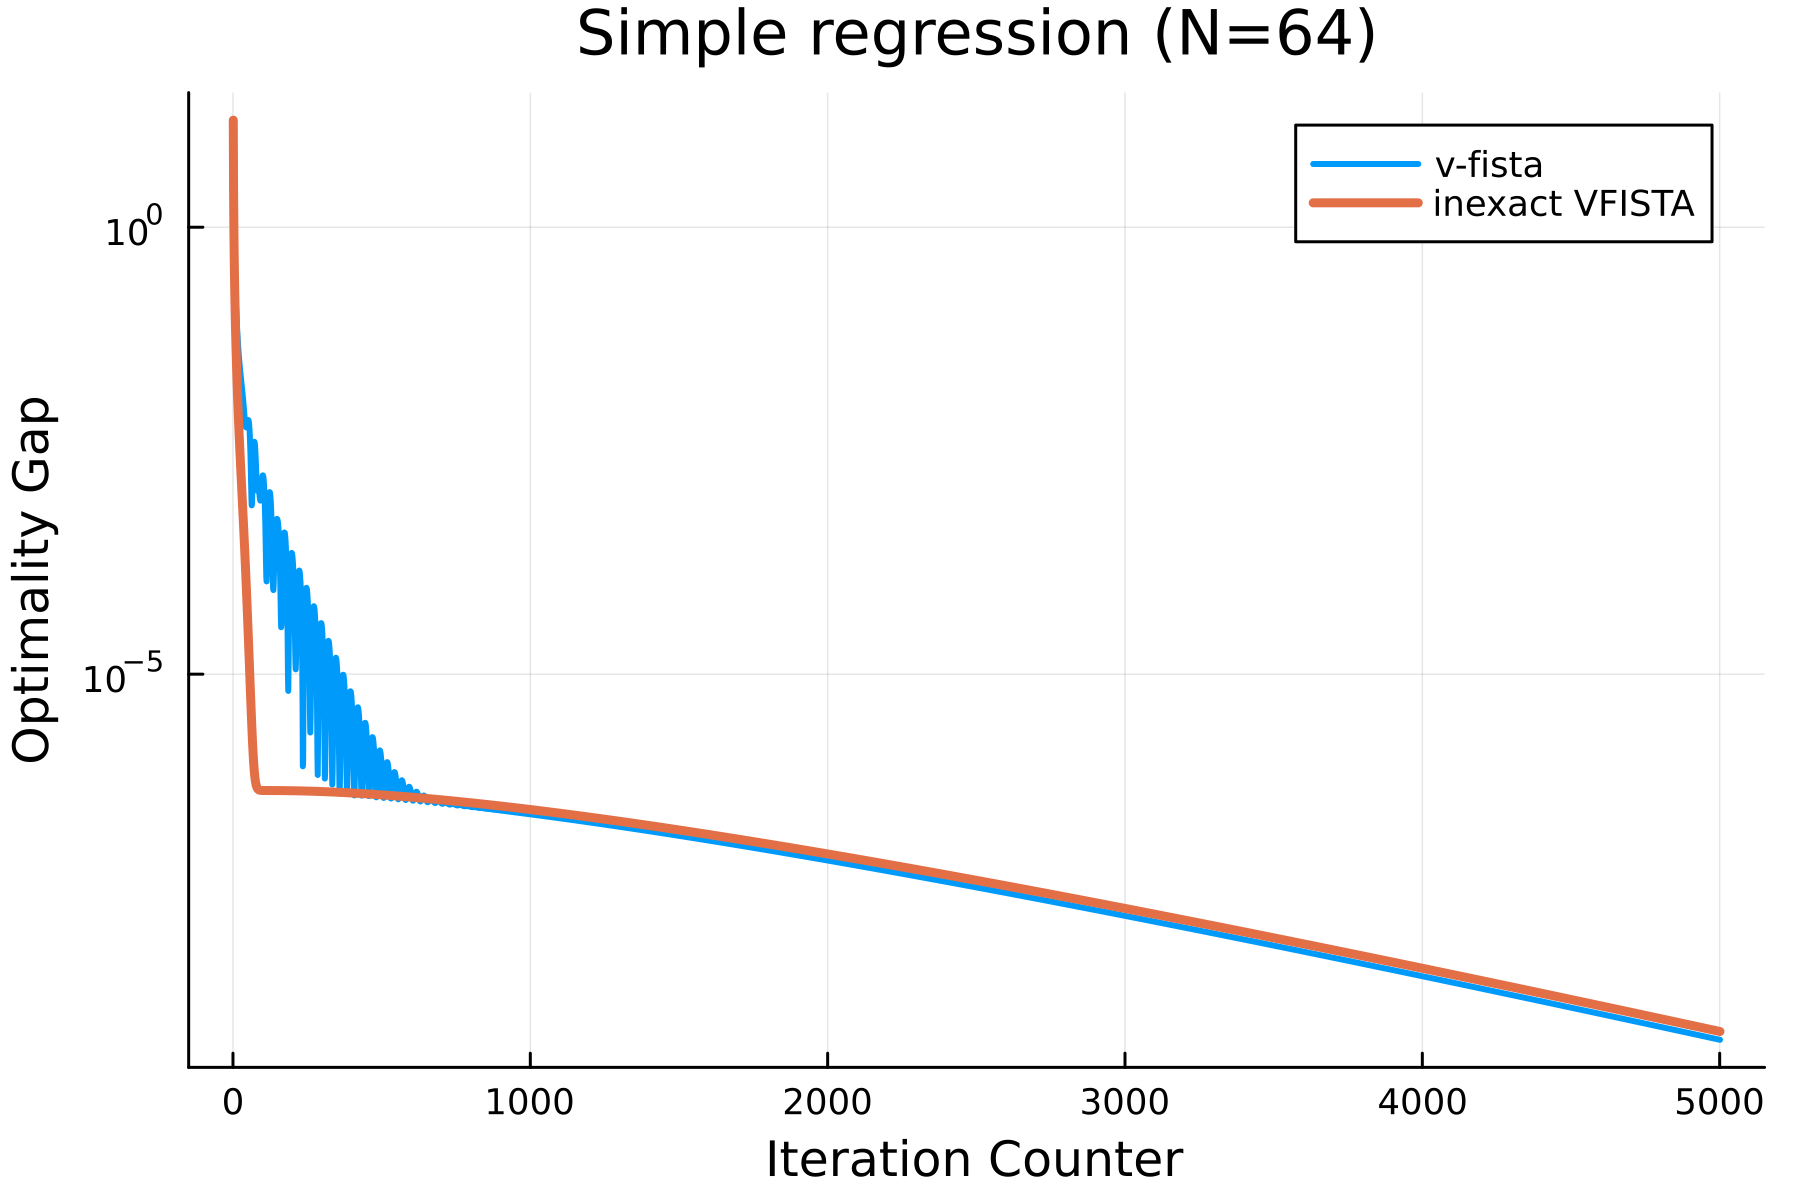
\includegraphics[width=\textwidth]{assets/simple_regression_loss_64.png}
                \caption{Optimality gap $h(x_k)$ on log scale. The x-axis is the iteration counter. }
                \label{fig:simple-regression-optimality-gap-64}
            \end{subfigure}
            ~
            \begin{subfigure}[b]{0.47\textwidth}
                \centering
                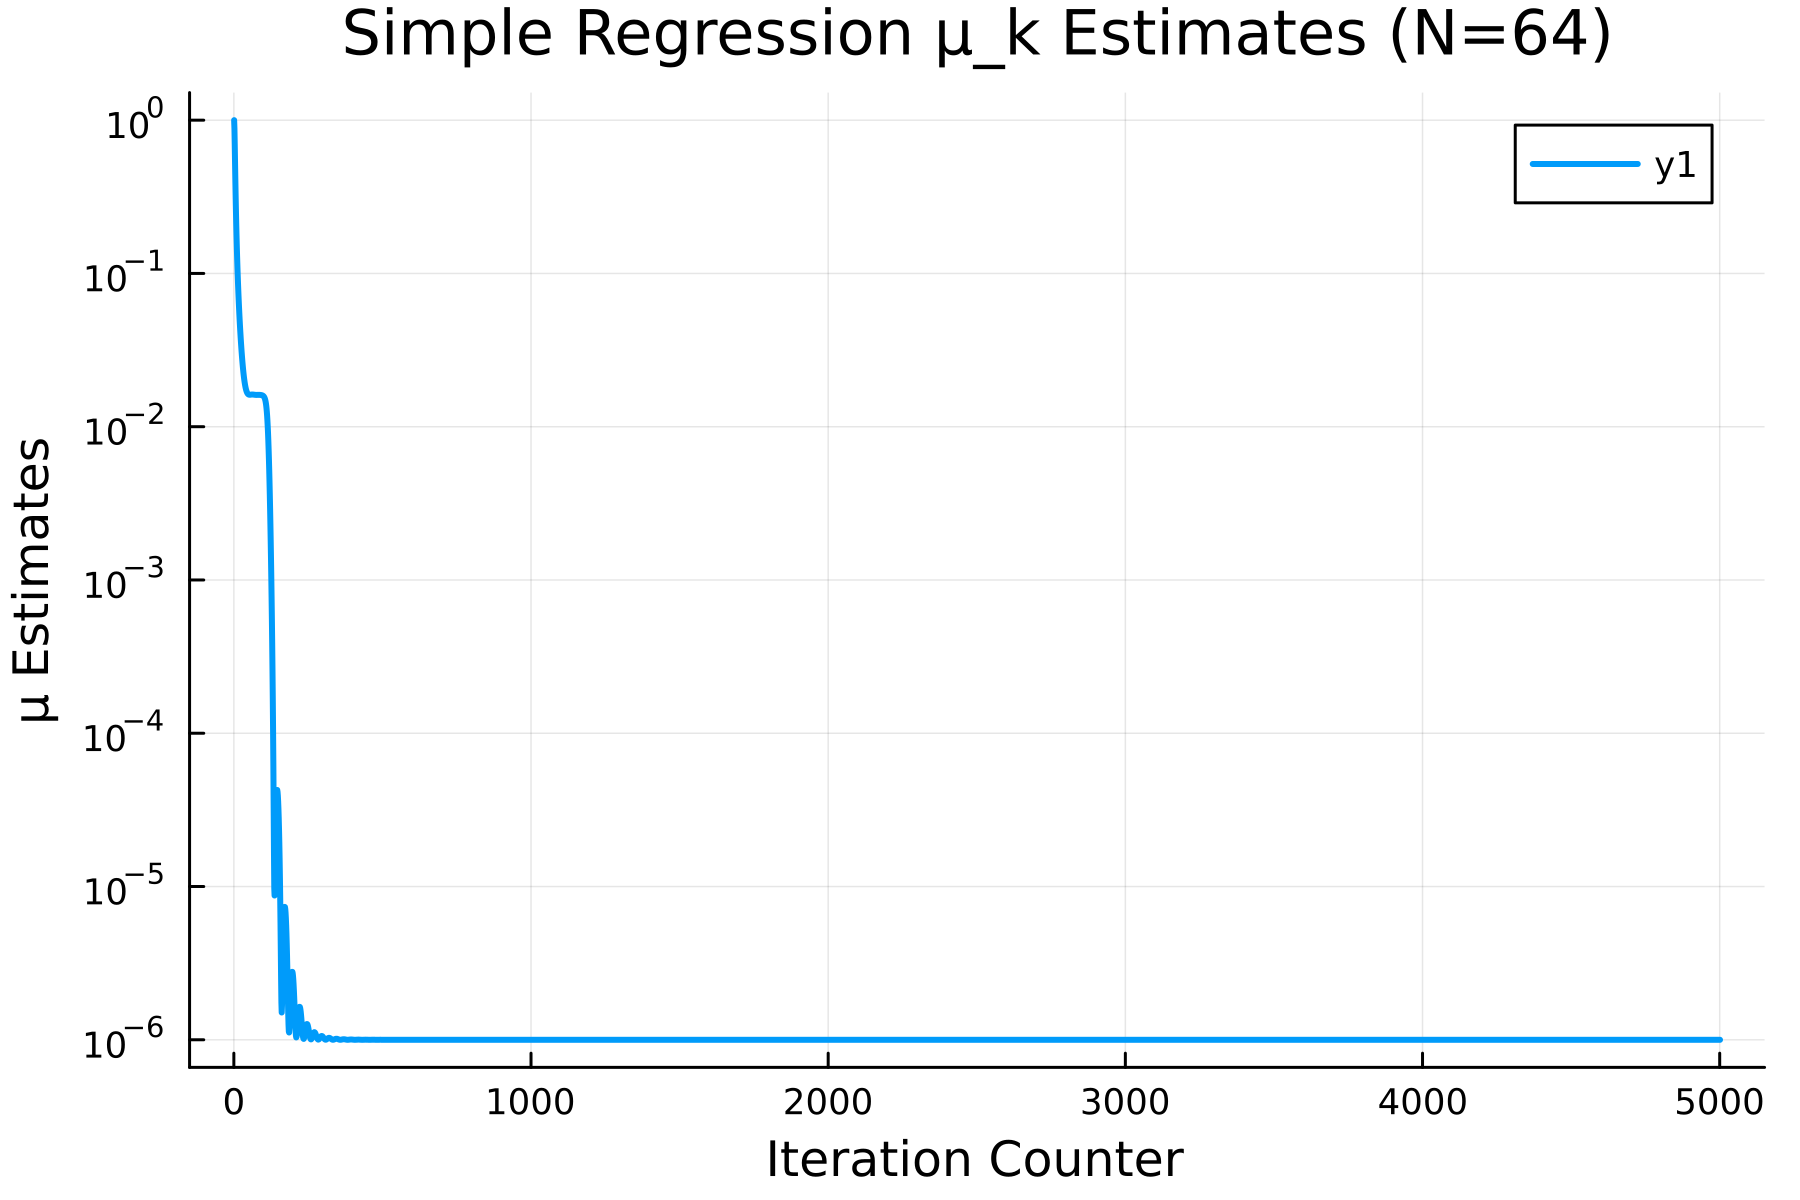
\includegraphics[width=\textwidth]{assets/simple_regression_loss_sc_estimates_64.png}
                \caption{$\mu_k$ estimates on log scale. The y-axis is the iteration counter. }
                \label{fig:simple-regression-mu-estimates-64}
            \end{subfigure}
            \caption{Regression with $N=64$. }
            \label{fig:simple-regression-64}
        \end{figure}

        \begin{figure}[H]
            \centering
            \begin{subfigure}[b]{0.47\textwidth}
                \centering
                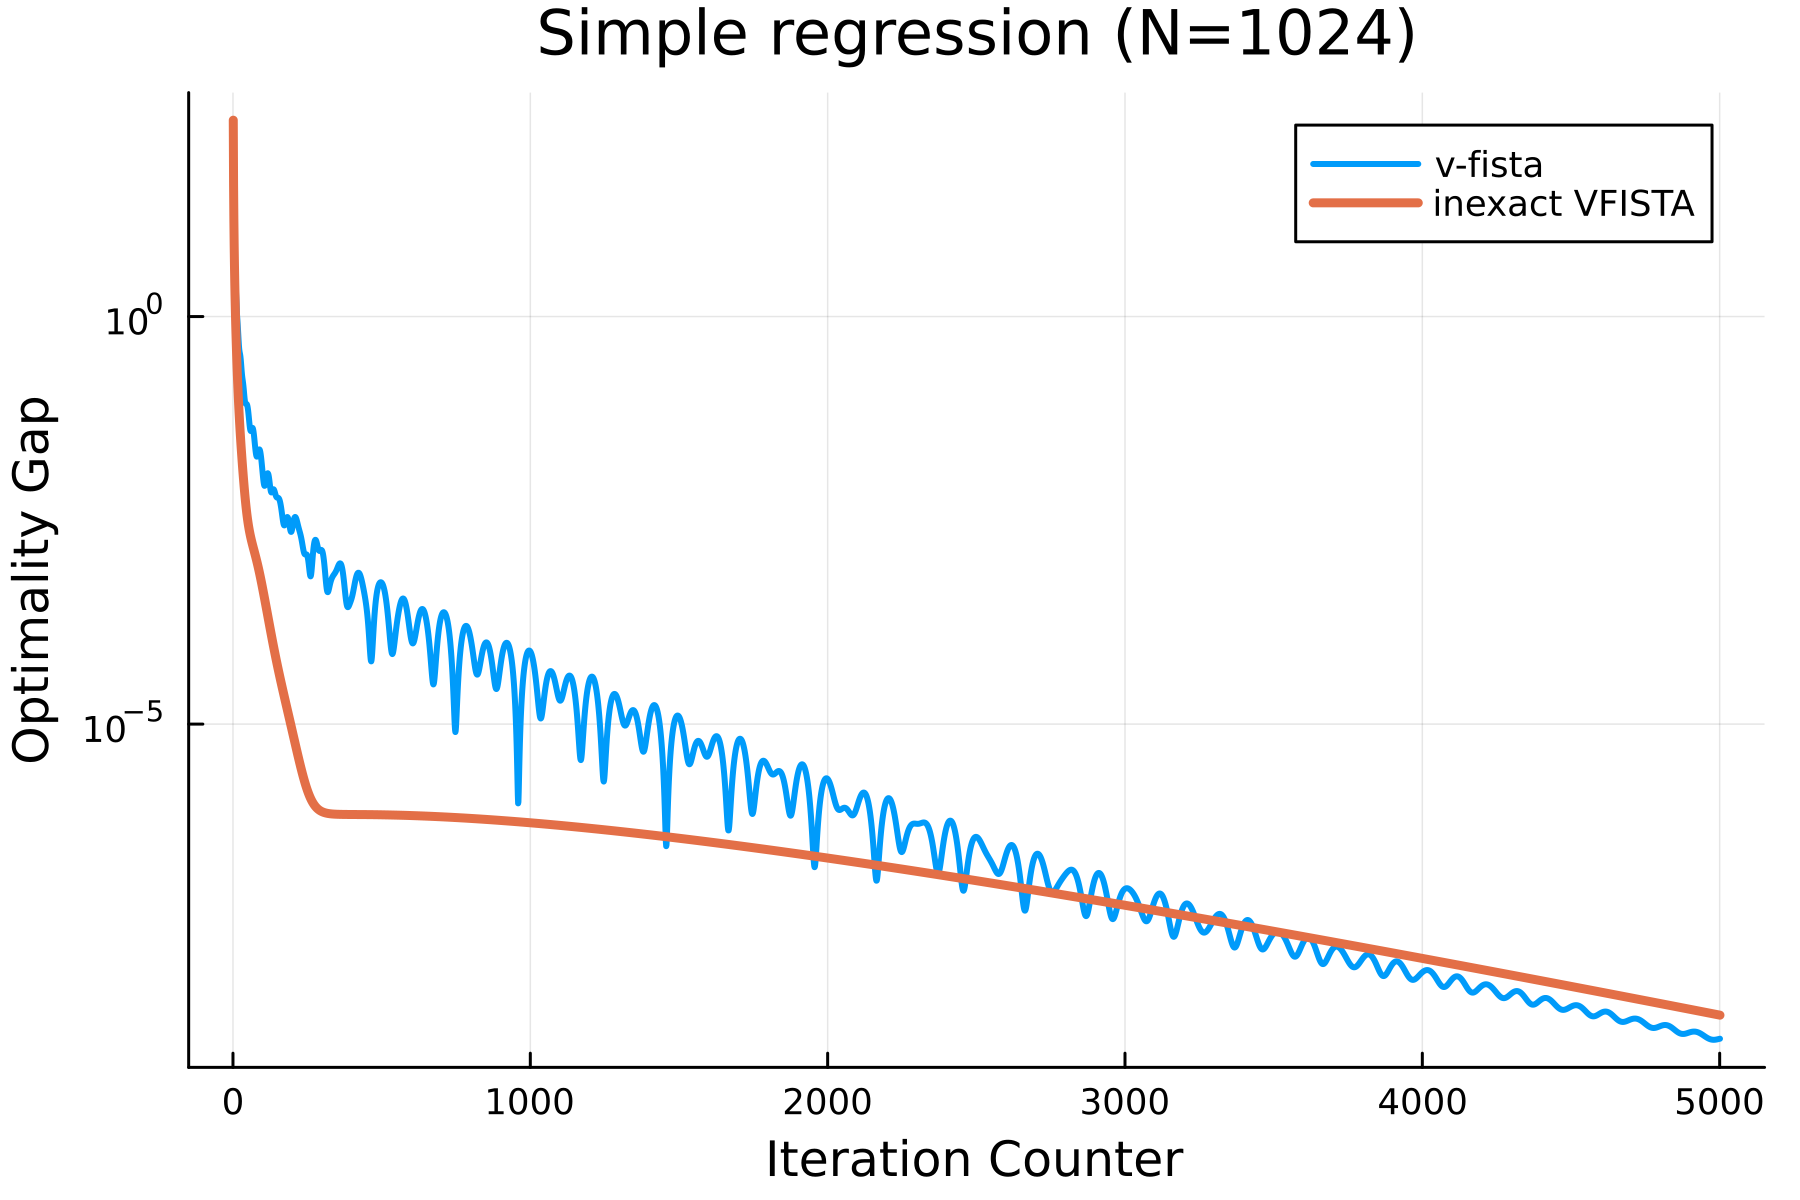
\includegraphics[width=\textwidth]{assets/simple_regression_loss_1024.png}
                \caption{Optimality gap $h(x_k)$ on log scale. The x-axis is the iteration counter. }
                \label{fig:simple-regression-optimality-gap-1024}
            \end{subfigure}
            ~ 
            \begin{subfigure}[b]{0.47\textwidth}
                \centering
                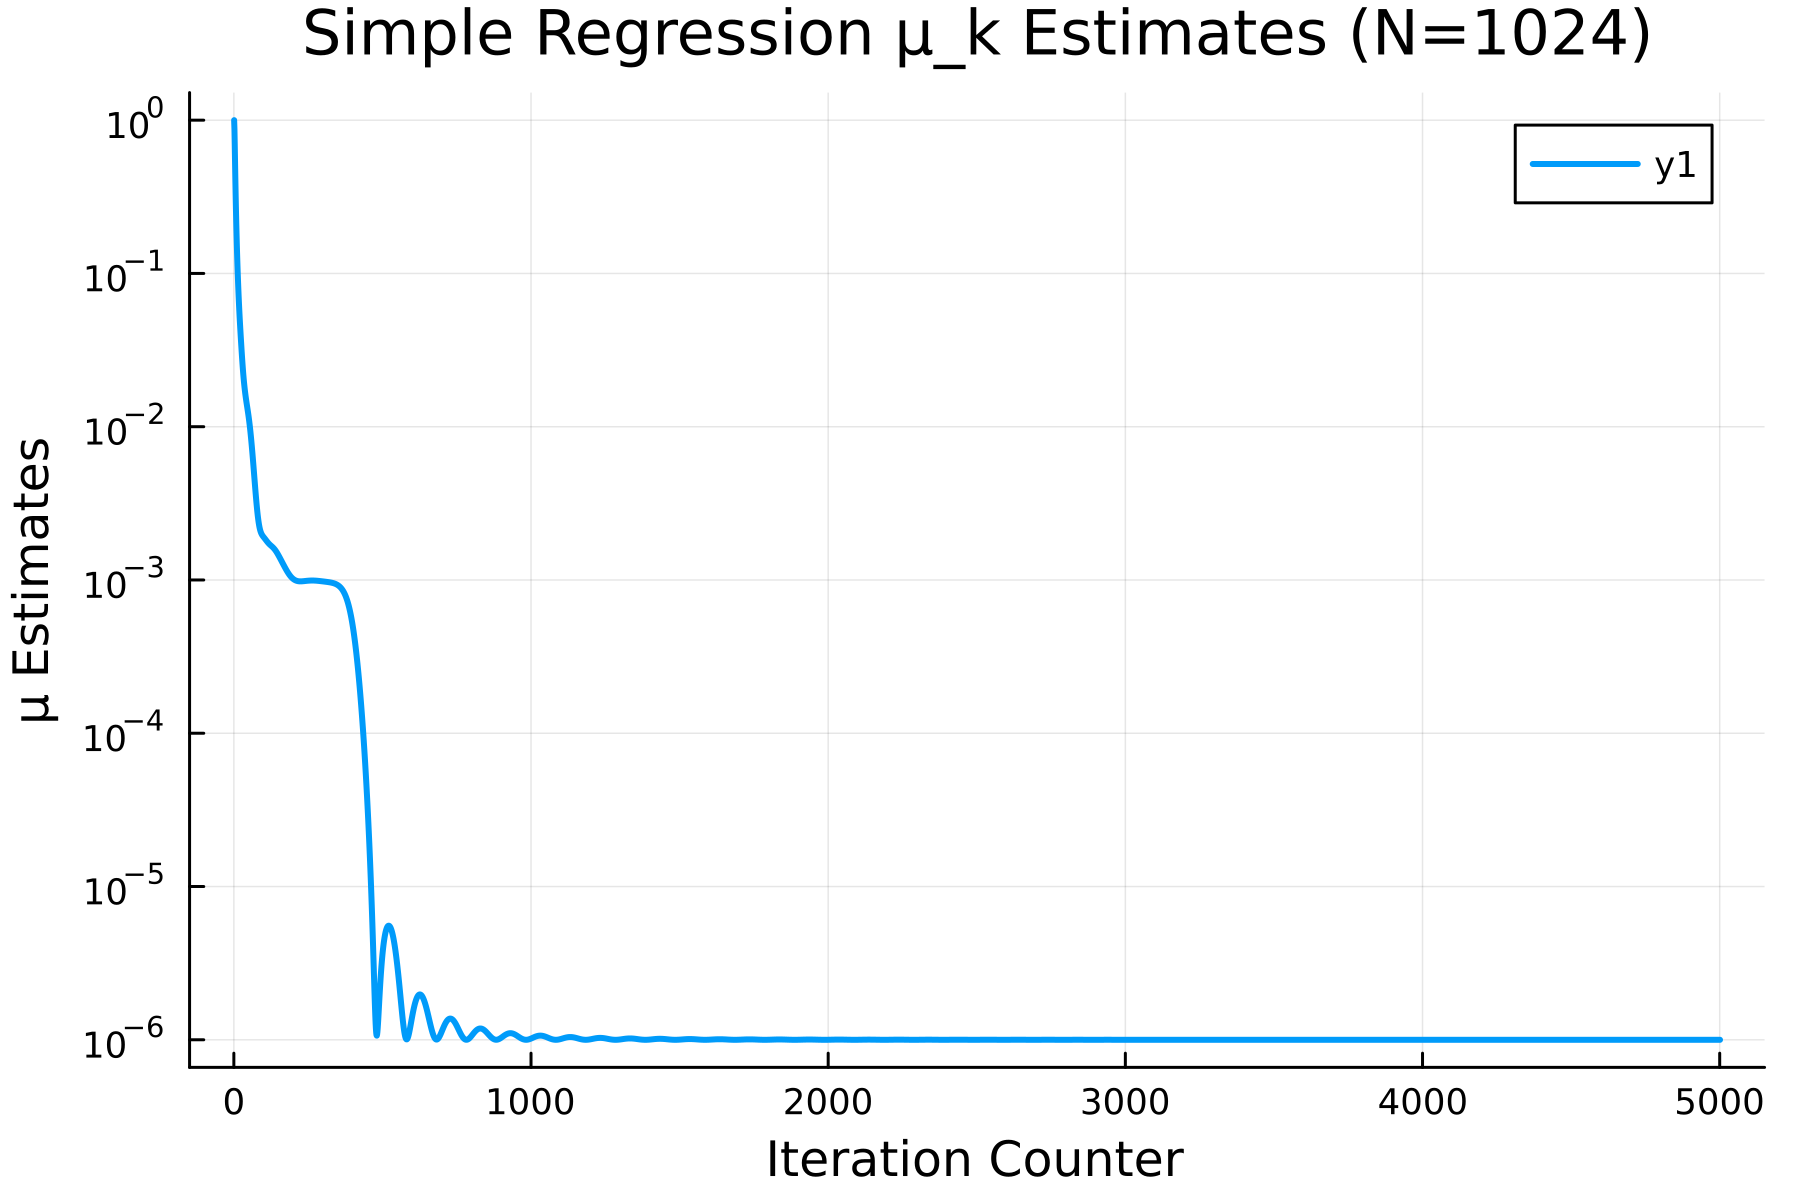
\includegraphics[width=\textwidth]{assets/simple_regression_loss_sc_estimates_1024.png}
                \caption{The $\mu_k$ estimates on log scale. The y-axis is the iteration counter. }
                \label{fig:simple-regression-mu-estimates-1024}
            \end{subfigure}
            \caption{Regression with $N=1024$. }
            \label{fig:simple-regression-1024}
        \end{figure}
       
        Our second experiment is conducted using the LASSO problem where the objective function is the composite $h$ given by
        \begin{align*}
            f(x) &:= \frac{1}{2} \Vert Ax - b\Vert^2_2, 
            \\
            g(x) &:= \lambda \Vert x\Vert_1, 
            \\
            h(x) &:= f(x) + g(x). 
        \end{align*}
        For the setup of the numerical experiments: 
        \begin{enumerate}
            \item $A\in \RR^{N\times N}$ is a dense matrix of Gaussian random variable $\mathcal N(0, 1)$. 
            \item We set $\lambda=0.01$ the regularization parameter to be $0.1$ for both set of experiments. 
            \item We produced the vector $b$ by setting vector $x^+$ to be $x^+_k = \cos(2k\pi) + \epsilon_k$ where $k\in \N, \;0 \le k \le N-1$, and $b = Ax^+$ where $\epsilon_i \sim \mathcal N(0, 10^{-4})$. The vector $x^+$ is promptly discarded after making the vector $b$. 
            \item To estimate $L, \mu$ for V-FISTA, we choose $L = \Vert AA^T\Vert_2$, and $\mu = \Vert (A^TA)^{-1}\Vert^{-1}_2$ as the estimate. For inexact V-FISTA, we give $L=1, \mu_0 = 1/2$ as the initial estimate. 
        \end{enumerate}
        The optimality gap is estimated. 
        We estimated the minimum $f_*$ using the smallest value ever produced among all algorithms tested for 5000 iterations. 
        \hyperref[fig:lasso-experiment-64]{Figure \ref*{fig:lasso-experiment-64}} showed the convergence rate of when $N=64$ for against FISTA, V-FISTA, and Inexact V-FISTA. 
        \hyperref[fig:lasso-experiment-1024]{Figure \ref*{fig:lasso-experiment-1024}} showed the convergence rate of when $N=1024$ against FISTA, V-FISTA, and Inexact V-FISTA. 

        \begin{figure}[H]
            \centering
            \begin{subfigure}[b]{0.47\textwidth}
                \centering
                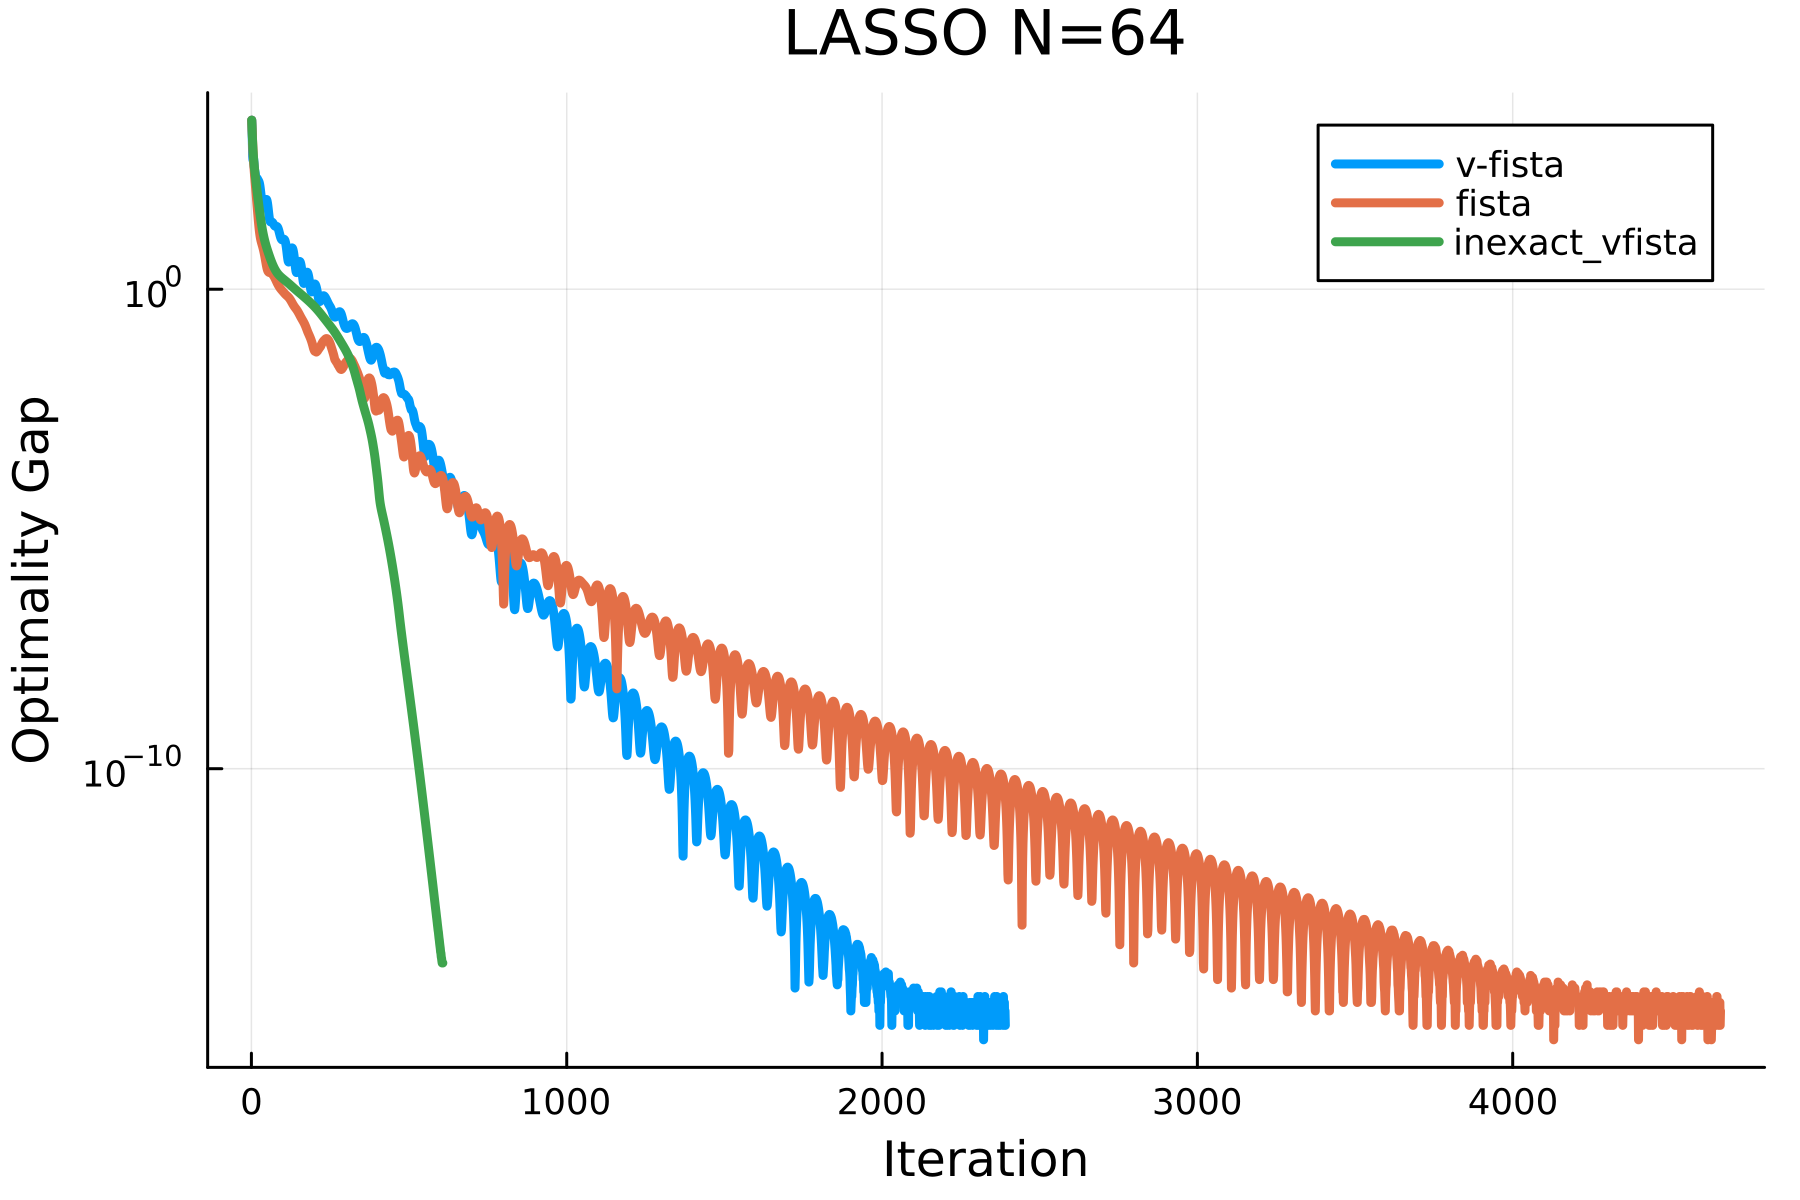
\includegraphics[width=\textwidth]{assets/lasso_loss_64.png}
                \caption{Optimality gap for LASSO with $N = 64$.}
            \end{subfigure}
            ~
            \begin{subfigure}[b]{0.47\textwidth}
                \centering
                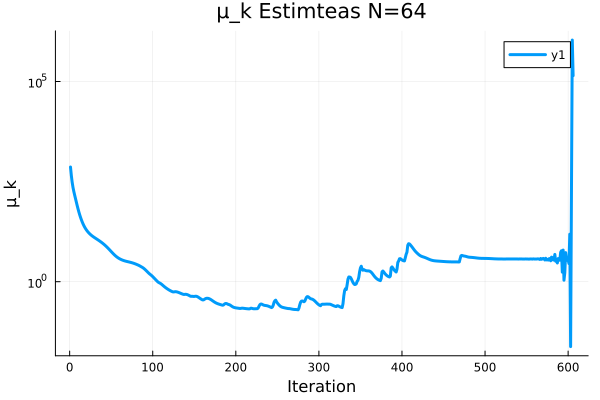
\includegraphics[width=\textwidth]{assets/lasso_sc_estimates_64.png}
                \caption{$\mu_k$ estimates for LASSO with $N = 64$.}
            \end{subfigure}
            \caption{Optimality gap and $\mu_k$ estimates. }
            \label{fig:lasso-experiment-64}
        \end{figure}

        \begin{figure}[H]
            \centering
            \begin{subfigure}[b]{0.47\textwidth}
                \centering
                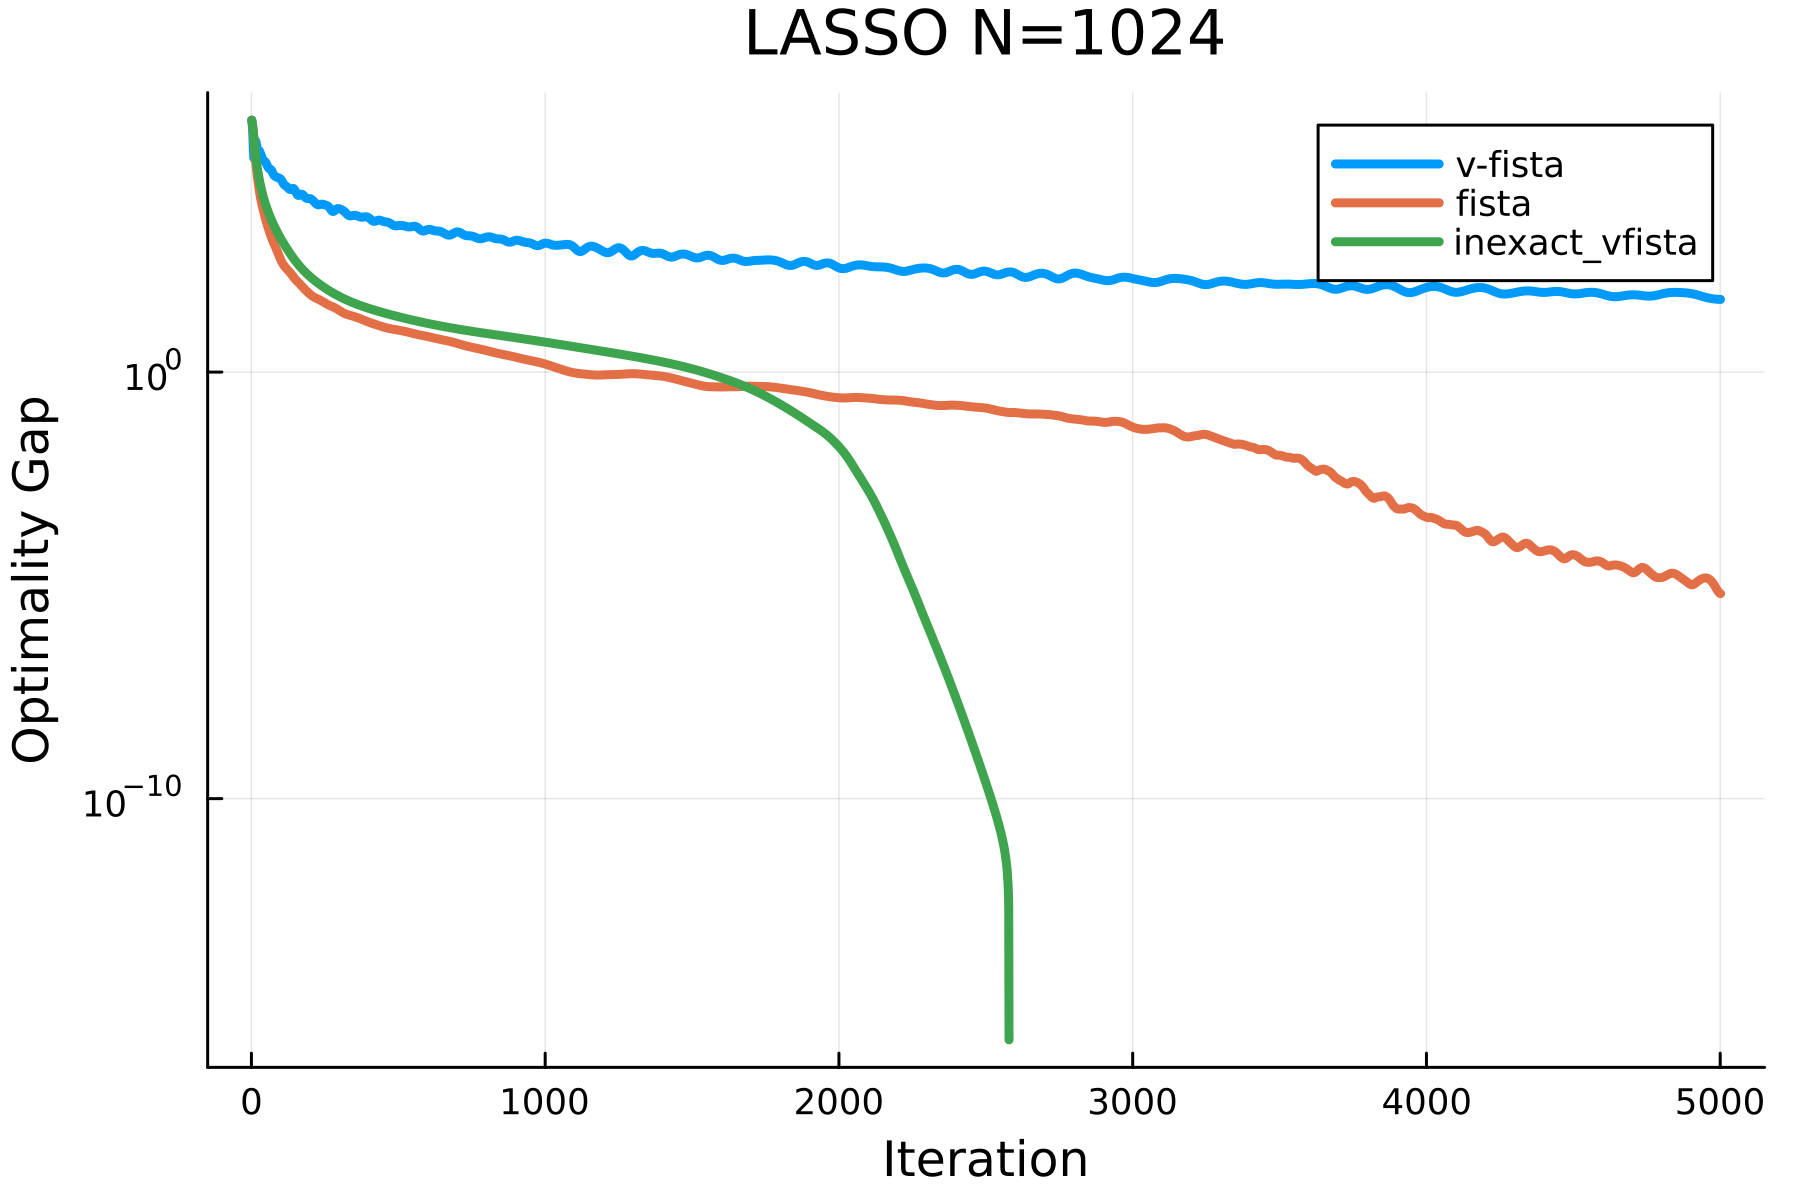
\includegraphics[width=\textwidth]{assets/lasso_loss_1024.png}
                \caption{Optimality gap for LASSO with $N = 1024$.}
            \end{subfigure}
            ~
            \begin{subfigure}[b]{0.47\textwidth}
                \centering
                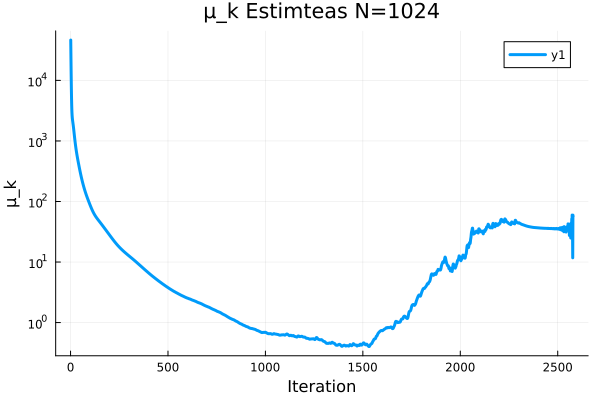
\includegraphics[width=\textwidth]{assets/lasso_sc_estimates_1024.png}
                \caption{$\mu_k$ estimates for LASSO with $N = 1024$.}
            \end{subfigure}
            \caption{Optimality gap and $\mu_k$ estimates. }
            \label{fig:lasso-experiment-1024}
        \end{figure}
    
    \subsection{Cannonical form of convex quadratic}\label{sec:cannonical-convex-quadratic}
        
    
    \subsection{Convergence analysis by eigensystem of the generalized matrix recurrences of Nesterov's acceleration}\label{sec:convergence-by-eigensystem}
        \subsubsection{Block diagonal linear recurrence matrix}
        \subsubsection{Eigensystem}
        \subsubsection{Spectral radius}
        \subsubsection{Worst Case Complexity}




% \printbibliography

\bibliographystyle{siam}
\bibliography{references/refs}

\appendix
\section{Postoned proofs}
    \subsection{Proof for \SCPPMAPG}\label{proof:derivations-SC-PPM-AGP}
        \begin{proof}
            (Proof of 
            \hyperref[def:SC-PPM-APG]
            {Definition \ref*{def:SC-PPM-APG}})
            \\
            The functions inside of ``argmin" is easy to solve because they are just quadratic functions. 
            We write it here for future verifications and a peace of the mind. 
            \begin{align*}
                x_{t + 1} &= \argmin_{x}\left\lbrace
                    \langle \mathcal G_L(y_t), x - y_t\rangle 
                    + 
                    \frac{\mu}{2}\Vert x - y_t\Vert^2 +  
                    \frac{1}{2\tilde \eta_{t}}\Vert x - x_t\Vert^2
                \right\rbrace
                \\
                \iff 
                \mathbf 0 & = 
                \mathcal G_L(y_t) + \mu(x - y_t) + \tilde \eta_{t}^{-1}(x - x_t)
                \\
                &= 
                \mathcal G_L(y_t) + (\mu + \tilde \eta_{t}^{-1}) x - \mu y_t - \tilde \eta_{t}^{-1} x_t
                \\
                \iff 
                (\mu + \tilde \eta_{t}^{-1})x 
                &= 
                \mu y_t + \tilde \eta_{t}^{-1} x_t - \mathcal G_L(y_t)
                \\
                \implies 
                x &= (\mu + \tilde \eta_{t}^{-1})^{-1 }
                (\mu y_t + \tilde \eta_{t}^{-1} x_t - \mathcal G_L(y_t)). 
            \end{align*}
            We can make the assumption that $\mu + \eta_{t}^{-1} > 0$ because $\tilde\eta_t > 0$. 
            Similarly for $y_{t + 1}$, it's solving a simple quadratic minimization problem, yielding: 
            \begin{align*}
                \mathbf 0 &= \mathcal G_L(y_t) + L(x - y_t) + \eta_{t + 1}^{-1}(x - x_{t + 1})
                \\
                &= (L + \eta_{t + 1}^{-1})x - L y_t - \eta_{t + 1}^{-1}x_{t + 1} + \mathcal G_L(y_t) 
                \\
                (L + \eta_{t + 1}^{-1})x &= 
                Ly_t + \eta_{t + 1}^{-1} x_{t + 1} - \mathcal G_L(y_t)
                \\
                \implies 
                x &= 
                (L\eta_{t + 1} + 1)^{-1}(L\eta_{t + 1}(y_t - L^{-1}\mathcal G_L(y_t)) + x_{t + 1}). 
            \end{align*}
            We had verified the results for the peace of the mind. 
        \end{proof}

    \subsection{Analysis of the forms}
        \begin{proposition}[SC Generic similar triangle]
            \label{prop:s-cvx-generic-sim-triangle-from-s-cvx-ppm-apg}
            \hyperref[def:SC-similar-triangle]
            {Definition \ref*{def:SC-similar-triangle}}
            is a special case of the 
            \hyperref[def:SC-PPM-APG]{Definition \ref*{def:SC-PPM-APG}}. 
            (\SCPPMAPG). 
            Suppose that $(x_t, y_t, z_t), \eta_t, \tilde \eta_t$ be the iterates and the stepsize sequences be given by the 
            \SCPPMAPG.
            If in addition, the sequence $\tilde \eta_t, \eta$ satisfies the conditions for all $t \in \N$
            \begin{align*}
                \tilde\eta_{t} &= \eta_t + L^{-1} + L^{-1} \mu \tilde\eta_{t}, 
            \end{align*}
            then $x_{t +1}$ in the the AG Generic Form has alternative representation: 
            \begin{align*}
                x_{t + 1} &= 
                z_{t + 1} + 
                \frac{L\eta_t}{1 + \mu \tilde \eta_{t}} 
                (z_{t + 1} - z_t). 
            \end{align*}
            This would at the end, produce the following relations for all $t \in \N$: 
            \begin{align*}
                z_{t + 1} &= 
                y_t - L^{-1}\mathcal G_L(y_t), 
                \\
                x_{t + 1}&= 
                z_{t + 1} + \frac{L\eta_t}{1 + \mu\tilde \eta_{t}}(z_{t + 1} - z_t), 
                \\
                y_{t + 1}&= 
                (1 + L\eta_{t + 1})^{-1} (L\eta_{t + 1}z_{t + 1} + x_{t + 1}). 
            \end{align*}
        \end{proposition}
        \begin{proof}
            We start by showing that there exists a constant $\alpha \in \RR$ such that $z_{t + 1} - z_t = \alpha (x_{t + 1} - z_{t + 1})$ by $\tilde \eta_{t} = \eta_t + L^{-1} + L^{-1} \mu \tilde \eta_{t}$. 
            Firstly, we have the equality which it's proved at the end. 
            \begin{align*}
                z_{t + 1} - z_t
                &= 
                - (L\eta_t)^{-1} y_t 
                - L^{-1}\mathcal G_L(y_t) + (L \eta_t)^{-1} x_t. 
                \tag{1}
            \end{align*}
            Next, we have this equality which we proved later at the end: 
            \begin{align*}
                x_{t + 1} - z_{t + 1}
                &= 
                (1 + \mu\tilde \eta_{t})^{-1}
                \left(
                    x_t - y_t +     
                    \left(
                        - \tilde \eta_{t} + L^{-1}
                        + \mu \tilde \eta_{t}L^{-1}
                    \right)
                    \mathcal G_L(y_t)
                \right).\tag{2} 
            \end{align*}
            Since 
            \begin{align*}
                \tilde\eta_{t} &= \eta_t + L^{-1} + L^{-1} \mu \tilde\eta_{t}
                \\
                (1 - L^{-1}\mu)\tilde \eta_{t}
                &= L^{-1} + \eta_t 
                \\
                - \tilde \eta_{t} + L^{-1}\mu \tilde \eta_{t}
                + L^{-1}
                &= - \eta_t, 
            \end{align*}
            so substituting 
            \begin{align*}
                x_{t + 1} - z_{t + 1}
                &= 
                (1 + \mu \tilde \eta_{t})^{-1}
                (x_t - y_t - \eta_t \mathcal G_L(y_t))
                \\
                &= (1 + \mu \tilde \eta_{t})^{-1}
                \eta_t(\eta_{t}^{-1}(x_t - y_t) - \mathcal G_L(y_t))
                \\
                &= (1 + \mu \tilde \eta_{t})^{-1}
                \eta_t L(z_{t + 1} - z_t)
                \\
                x_{t + 1} &= 
                z_{t + 1} + 
                \frac{L \eta_t}{1 + \mu \tilde \eta_t}(z_{t + 1} - z_t). 
            \end{align*}
            To show (1): 
            \begin{align*}
                y_{t} &= (1 + L\eta_{t})^{-1}(L\eta_{t}z_{t} + x_{t})
                \\
                (1 + L\eta_t)y_t - x_t &= L\eta_t z_t
                \\
                z_t & = (L\eta_t)^{-1}((1 + L\eta_t)y_t - x_t), 
                \\[1em]
                z_{t + 1} - z_t 
                &= \underbrace{ y_t - L^{-1}\mathcal G_L(y_t)}_{=z_{t + 1}}
                - \underbrace{(L\eta_t)^{-1}((1 + L\eta_t)y_t - x_t)}_{=z_t}
                \\
                &= 
                y_t - L^{-1} \mathcal G_L(y_t) - (L\eta_t)^{-1}y_t - y_t + (L\eta_t)^{-1} x_t
                \\
                &= 
                -L^{-1}\mathcal G_L(y_t) + (L\eta_t)^{-1}(x_t - y_t)
                \\
                &= 
                L^{-1}(\eta_t^{-1}(x_t - y_t) -\mathcal G_L(y_t)). 
            \end{align*}
            To show (2): 
            \begin{align*}
                x_{t + 1} - z_{t + 1}&= 
                \left(
                    (1 + \mu \tilde \eta_{t})^{-1} (\mu \tilde \eta_{t }y_t + x_t)
                    - \frac{\tilde \eta_{t }}{1 + \mu\tilde \eta_{t }}
                    \mathcal G_L(y_t)
                \right) - \left(
                    y_t - L^{-1}\mathcal G_L(y_t)
                \right)
                \\
                &= 
                (1 + \mu \tilde \eta_{t})^{-1}
                \left(
                    x_t + \mu \tilde \eta_{t} y_t
                    - \tilde \eta_{t} \mathcal G_L(y_t)
                    - (1 + \mu \tilde \eta_{t})
                    (y_t - L^{-1}\mathcal G_L(y_t))
                \right)
                \\
                &= 
                (1 + \mu\tilde \eta_{t})^{-1}
                \left(
                    x_t - y_t + 
                    (
                        -\tilde \eta_{t} + 
                        (1 + \mu\tilde \eta_{t})L^{-1}
                    )
                    \mathcal G_L(y_t)
                \right)
                \\
                &= 
                (1 + \mu\tilde \eta_{t})^{-1}
                \left(
                    x_t - y_t +     
                    (
                        - \tilde \eta_{t} + L^{-1}
                        + \mu \tilde \eta_{t}L^{-1}
                    )
                    \mathcal G_L(y_t)
                \right). 
            \end{align*}
        \end{proof}

        \begin{proposition}[Momentum form is equivalent to Similar Triangle form]
            \label{prop:momentum-equiv-to-similar-triangle}
            \;\\
            Let iterates $(x_t, y_t, z_t), \eta_t, \tilde \eta_t$ be given by the relations in 
            \hyperref[def:SC-similar-triangle]
            {Definition \ref*{def:SC-similar-triangle}}
            then it's algebraically equivalent to: 
            \begin{align*}
                y_{t + 1} &= z_{t + 1} + 
                \frac{L\eta_t}{(1 + \mu \tilde\eta_{t})(1 + L\eta_{t + 1})}(z_{t + 1} - z_t)
                \\
                z_{t + 1} &= y_t - L^{-1}\mathcal G_L(y_t). 
            \end{align*}
            Which fits
            \hyperref[def:generic-nesterov-momentum-form]
            {Definition \ref*{def:generic-nesterov-momentum-form}}
            with 
            $$
                \theta_{t + 1} = \frac{L\eta_t}{(1 + \mu \tilde\eta_{t})(1 + L\eta_{t + 1})}.
            $$
        \end{proposition}
        \begin{proof}
            From the similar triangle form, directly substituting the value of $x_{t + 1}$ into the expression for $y_{t + 1}$ it yields: 
            \begin{align*}
                y_{t + 1} &= 
                (1 + L\eta_{t + 1})^{-1} (L\eta_{t + 1}z_{t + 1} + x_{t + 1})
                \\
                &= 
                (1 + L\eta_{t + 1})^{-1}
                \left(
                    L\eta_{t + 1}z_{t + 1} + z_{t + 1} + \frac{L\eta_t}{1 + \mu\tilde \eta_t}(z_{t + 1} - z_t)
                \right)
                \\
                &= 
                (1 + L\eta_{t + 1})^{-1}
                \left(
                    (1 + L\eta_{t + 1})z_{t +1} + 
                    \frac{L\eta_t}{1 + \mu\tilde \eta_t}(z_{t + 1} - z_t)
                \right)
                \\
                &= 
                z_{t + 1} + 
                \frac{L\eta_t}{(1 + L\eta_{t + 1})(1 + \mu\tilde \eta_t)}
                (z_{t + 1} - z_t)
            \end{align*}
        \end{proof}
        
        \begin{proposition}[Chambolle Dossal as an instance of Similar Triangle Form]
            \label{prop:cham-dossal-2015-is-similar-triangle}
            \;\\
            Let iterates $(x_t, y_t, z_t)$ and stepszie sequence $\tilde \eta_t, \eta_t$ be generated by SC Generic Similar Triangle form
            (\hyperref[def:SC-similar-triangle]
            {Definition \ref*{def:SC-similar-triangle}}). 
            Then the algorithm are equivalent to Chambolle and Dossal 2015 algorithms 
            (\hyperref[def:chambolle-dossal-2015]
            {Definition \ref*{def:chambolle-dossal-2015}})
            if and only if we have sequence $t_n = L \tilde \eta_{n}$ and $\mu = 0$. 
        \end{proposition}
        \begin{proof}
            First, we present $\eta_t$ using $\tilde \eta_t$. 
            The Generic Similar Triangle Form admits has $x_{t + 1}$ to be: 
            \begin{align*}
                x_{t + 1} 
                &= z_{t + 1} + (1 + \mu\tilde \eta_{t})^{-1}L\eta_t (z_{t + 1} - z_t)
                \\
                &=  
                (1 + L\eta_t(1 + \mu \tilde \eta_{t})^{-1})z_{t + 1}
                - L\eta_t(1 + \mu\tilde \eta_{t})^{-1} z_t
                \\
                &= 
                \left(
                    \frac{1 + \mu\tilde \eta_{t} + L \eta_t}{1 + \mu \tilde \eta_{t}}
                \right)z_{t + 1}
                + 
                z_t - 
                \left(
                    1 + \frac{ L\eta_t}{\mu \tilde \eta_t + 1}
                \right)z_t
                \\
                & 
                \textcolor{gray}{
                    \text{use: } \tilde \eta_t = \eta_t + L^{-1} + L^{-1}\mu\tilde \eta_t
                }
                \\
                &= 
                \left(
                    \frac{L\tilde \eta_{t}}{1 + \mu\tilde \eta_{t}}
                \right)z_{t + 1}
                + 
                z_t 
                - 
                \left(
                    \frac{L\tilde \eta_{t}}{1 + \mu \tilde \eta_{t}}
                \right)z_t 
                \\
                &= z_t + 
                \left(
                    \frac{L\tilde \eta_{t}}{1 + \mu \tilde \eta_{t}}
                \right)
                (z_{t + 1} - z_t). 
            \end{align*}
            Recall that Chmabolle Dossal 2015 has $x_{n + 1} = z_t + t_n(z_{t + 1} - z_t)$, 
            therefore above suggests that $t_n = L \tilde \eta_{n}(1 + \mu \tilde \eta_{n})^{-1}$. 
            From the second equality to the third equality, we use the relations $L\tilde \eta_{t} = \eta_t + 1 + \mu\tilde \eta_{t}$.
            At the same time, we check that: 
            \begin{align*}
                y_{t + 1} &= \left(
                    \frac{L\eta_{t + 1}}{1 + L \eta_{t + 1}}
                \right)z_{t + 1} + 
                \left(
                    \frac{1}{1 + L \eta_{t + 1}}
                \right) x_{t + 1}
                \\
                &= 
                \left(
                    1 - \frac{1}{1 + L\eta_{t + 1}}
                \right)z_{t + 1} + 
                \left(
                    \frac{1}{1 + L \eta_{t + 1}}
                \right)x_{t + 1}. 
            \end{align*}
            Recall that in Chambolle Dossal 2015, itertes $y_{n + 1} = (1 - t_{n + 1}^{-1})z_{n + 1} + t_{n + 1}^{-1} x_{n + 1}$. 
            Therefore, the above results suggests that $t_{n + 1} = 1 + L\eta_{n + 1}$. 
            However, by the relations between $\tilde \eta_n, \eta_n$ as asserted via the similar triangle form, we have 
            \begin{align*}
                \tilde \eta_t &= \eta_t + L^{-1} + L^{-1}\mu \tilde \eta_t
                \\
                \iff 
                L\tilde \eta_t - \mu \tilde \eta_t 
                &= 
                L \eta_t + 1
                \\
                \iff 
                (L - \mu)\tilde \eta_t &= L\eta_t + 1. 
            \end{align*}
            For $t_n$ to be the same, these two have to be equivalent, but for all $\mu > 0$
            \begin{align*}
                L\tilde \eta_n (1 + \mu \tilde \eta_n)^{-1} \not = 
                (L - \mu )\tilde \eta_n. 
            \end{align*}
            Therefore, they are only equivalent when $\mu = 0$, then the generic similar triangle algorithm would be equivalently represented as the algrithm in Chambolle Dossal 2015's paper. 
        \end{proof}
        \begin{proposition}[V-FISTA is Similar Triangle Method]
        \label{prop:vfista-parameter-math}
            V-FISTA 
            (\hyperref[def:v-fista]{Definition \ref*{def:v-fista}}
            ) is a form of Generic Similar Triangle Form, where the stepsizes $\tilde \eta_t, \eta_t$ are constants: 
            \begin{align*}
                \tilde \eta_t 
                &= \frac{1}{\mu(\sqrt{\kappa} - 1)}
                \quad \forall t \in \N, 
                \\
                \eta_t
                &= 
                \frac{1}{\mu\sqrt{\kappa}}
                \quad \forall t \in \N. 
            \end{align*}
            This choice of step size sequences simplifies it to:
            \begin{align*}
                y_{t + 1} &= z_{t + 1} + 
                \frac{\sqrt{\kappa} - 1}{\sqrt{\kappa} + 1}
                (z_{t +1} - z_t), 
                \\
                z_{t + 1} 
                &= y_t - L^{-1}\mathcal G_L(y_t). 
            \end{align*}
        \end{proposition}
        \begin{proof}
            Suppose that $(\rho_t)_{t \in \N}$ is a sequence such that $\rho_t > 1$ for all $t$. 
            Consider for all $t \in \N$, the following relations between $\rho_t$ and $\tilde \eta_t, \eta_t$: 
            \begin{align*}
                L \eta_t &:= \rho_t, 
                \\
                \mu \tilde \eta_t &:= \frac{1}{\rho_t - 1}, 
                \\
                L \tilde \eta_t &:= \frac{\rho_t^2}{\rho_t - 1}. 
            \end{align*}
            Then it satisfies the of similar triangle $\tilde \eta_t = \eta_t + L^{-1} + L^{-1} \mu \tilde \eta_t$ because: 
            \begin{align*}
                L \tilde \eta_t - \mu \tilde \eta_t 
                &= \frac{\rho_t^2}{\rho_t - 1} - \frac{1}{\rho_t - 1}
                \\
                &= \frac{\rho_t^2 - 1}{\rho_t - 1} 
                \\
                &= \frac{(\rho_t - 1)(\rho_t + 1)}{\rho_t - 1} 
                \\
                &= \rho_t + 1
                \\
                &= L\eta_t + 1
            \end{align*}
            So by 
            \hyperref[prop:momentum-equiv-to-similar-triangle]{Proposition \ref*{prop:momentum-equiv-to-similar-triangle}}, 
            the momentum coefficient can be similified as well: 
            \begin{align*}
                \theta_{t + 1} 
                &= \frac{L\eta_t}{(1 + \mu \tilde\eta_{t})(1 + L\eta_{t + 1})}
                \\
                &= \frac{\rho_t}{
                    \left(
                        1 + \frac{1}{\rho_t - 1}
                    \right)
                    (1 + \rho_t)
                }
                \\
                &= \frac{\rho_t}{
                    \left(
                    \frac{\rho_t}{\rho_t - 1}
                    \right)
                    (1 + \rho_t)
                }
                \\
                &= 
                \frac{\rho_t - 1}{\rho_t}
                \frac{\rho_t}{1 + \rho_t}
                \\
                &= \frac{\rho_t - 1}{1 + \rho_t}. 
            \end{align*}
            Set $\rho_t = \sqrt{\kappa} \ge 1$, then we obtain the desired result, which is the V-FISTA algorithm. 
        \end{proof}
    \subsection{Lyapunov analysis proof continued}\label{sec:st2p_proof_continued}
        \textbf{Proof for Equation (\ref*{eqn:st2p-1}, \ref*{eqn:st2p-2})}:
        \\
        Fix any $k \in \N\cup \{0\}$, apply
        \hyperref[lemma:grad_map_linearization]
        {Lemma \ref*{lemma:grad_map_linearization}}
        with $z = z_{k + 1}, x = x_+$: 
        \begin{align*}
            \Delta_k &= h(z_{k + 1}) - h(x_+) = h(\mathcal T_L y_k) - h(x_+) 
            \\
            &\le 
            - \langle \mathcal G_l y_k, x_+ - y_k \rangle 
            - \frac{L}{2}\Vert L^{-1} \mathcal G_Ly_k\Vert^2
            \\
            &= 
            - \langle \mathcal G_l y_k, x_+ - y_k \rangle 
            - \frac{1}{2L}\Vert \mathcal G_L y_k\Vert^2
            \\
            \iff 
            0& \ge \Delta_k + \langle \mathcal G_L y_k, x_+ - y_k\rangle + \frac{1}{2L}\Vert \mathcal G_L y_k\Vert^2. 
        \end{align*}
        Similarly, by setting $z = z_{k + 1}, x = z_k$, it gives 
        \begin{align*}
            \Delta_k - \Delta_{k - 1} &= 
            h(z_{k + 1}) - h(x_+) - (h(z_k) - h(x_+)) 
            \\
            &= h(z_{k + 1}) - h(z_k)
            \\
            &= h( \mathcal G_L y_k) - h(z_k)
            \\
            &\le 
            - \langle \mathcal G_L y_k, z_k - y_k\rangle - 
            \frac{1}{2L} \Vert \mathcal G_L y_k \Vert^2
            \\
            \iff 
            0 &\ge
            \Delta_k - \Delta_{k - 1}
            + \langle \mathcal G_L y_k, z_k - y_k\rangle
            + \frac{1}{2L} \Vert \mathcal G_L y_k \Vert^2.
        \end{align*}
        \\
        \textbf{Proof for (\ref*{eqn:st2p-3})}: 
        \\
        Assume that $\sigma_k - \sigma_{k -1} \le \epsilon_k$ where $\epsilon_k \ge 0$ then for all $k \in \N$: 
        \begin{align*}
            &
            \sigma_k \Delta_k - \sigma_{k - 1} \Delta_{k - 1}
            \\
            & 
            \textcolor{gray}{
                \text{by: } \sigma_k - \sigma_{k - 1} \le \epsilon_k, \epsilon_k \ge 0
            }
            \\
            &\le 
            \sigma_k \Delta_k - (\sigma_k - \epsilon_k)\Delta_{k - 1}
            \\
            &= 
            (\sigma_k - \epsilon_k)\Delta_k - (\sigma_k - \epsilon_k)\Delta_{k - 1}
            + \epsilon \Delta_k 
            \\
            &= (\sigma_k - \epsilon_k)(\Delta_k - \Delta_{k - 1}) + \epsilon_k \Delta_k. 
        \end{align*}
        \\
        \textbf{Proof for (\ref*{eqn:st2p-4})}:
        \\
        Using the relations of the iterates as defined by the algorithm, it has $\forall k \in \N\cup \{0\}$
        \begin{align*}
            & \frac{1}{2} 
            \left(
                \Vert x_{k + 1} - x_+\Vert^2
                - 
                \Vert x_k - x_+\Vert^2 
            \right)
            \\
            &=
            \frac{1}{2} 
            \left(
                \Vert x_k - \tilde \eta_k\mathcal G_L (y_k) - x_+ \Vert^2 
                - 
                \Vert x_k - x_+\Vert^2
            \right)
            \\
            &= 
            \frac{1}{2}\left(
                -2\langle \tilde \eta_k \mathcal G_L(y_k), x_k - x_+\rangle
                + 
                \tilde \eta_k^2 \Vert \mathcal G_L(y_k)\Vert^2
            \right)
            \\
            &= 
            \langle \tilde \eta_k \mathcal G_L(y_k), x_k - x_+\rangle
                + 
            \frac{\tilde \eta_k^2}{2} \Vert \mathcal G_L(y_k)\Vert^2. 
        \end{align*}
        \\
        \textbf{Proof for (\ref*{eqn:st2p-5})}:
        \\
        To show $(\sigma_k - \epsilon_k)(\ref*{eqn:st2p-2}) + \epsilon_k(\ref*{eqn:st2p-1}) \le 0$, assume $\sigma_k - \epsilon_k \ge 0$, $\epsilon_k \ge 0$, so: 
        {\footnotesize
        \begin{align*}
            (\sigma_k - \epsilon_k)
            \left(
                \Delta_k - \Delta_{k - 1}
                + \langle \mathcal G_L y_k, z_k - y_k\rangle
                + \frac{1}{2L} \Vert \mathcal G_L y_k \Vert^2
            \right)
            + 
            \epsilon_k 
            \left(
                \Delta_k + \langle \mathcal G_L y_k, x_+ - y_k\rangle + \frac{1}{2L}\Vert \mathcal G_L y_k\Vert^2
            \right)
            &\le 
            0
            \\
            \iff
            (\sigma_k - \epsilon_k)(\Delta_k - \Delta_{k - 1}) 
            + \epsilon_k \Delta_k 
            + 
            \left(
                \langle \mathcal G_L y_k, 
                    (\sigma_k - \epsilon_k)(z_k - y_k)
                    + 
                    \epsilon_k (x_+ - y_k)
                \rangle
                + 
                \frac{\sigma_k}{2L}\Vert \mathcal G_Ly_k\Vert^2
            \right) 
            &\le 0
            \\
            \iff
            (\sigma_k - \epsilon_k)(\Delta_k - \Delta_{k - 1}) 
            + \epsilon_k \Delta_k 
            + 
            \left(
                \langle \mathcal 
                    G_L y_k, 
                    (\sigma_k - \epsilon_k)z_k + 
                    (\epsilon_k - \sigma_k - \epsilon_k)y_k
                    + 
                    \epsilon_k x_+
                \rangle
                + 
                \frac{\sigma_k}{2L}\Vert \mathcal G_Ly_k\Vert^2
            \right) 
            &\le 0
            \\
            \iff
            (\sigma_k - \epsilon_k)(\Delta_k - \Delta_{k - 1}) 
            + \epsilon_k \Delta_k 
            + 
            \left(
                \langle \mathcal 
                    G_L y_k, 
                    (\sigma_k - \epsilon_k)z_k - \sigma_k y_k + \epsilon_k x_+
                \rangle
                + 
                \frac{\sigma_k}{2L}\Vert \mathcal G_Ly_k\Vert^2
            \right) 
            &\le 0. 
        \end{align*}
        }

    

\end{document}
